% Working draft, 16 October 2026. Target: ISPCS 2027.
% Venue rules and submission requirements remain to be confirmed.
% All plotted data are embedded below; no auxiliary project files are required.
\documentclass[conference]{IEEEtran}
\usepackage{amsmath,amssymb,booktabs}
\usepackage{pgfplots}
\pgfplotsset{compat=1.18}
\usepackage[hidelinks]{hyperref}
\newcommand{\unit}[1]{\,\mathrm{#1}}
\newcommand{\clip}{\operatorname{clip}}
\title{tinyPTP: Hardware-Timestamped Clock Synchronization on Arduino Microcontrollers}
\author{\IEEEauthorblockN{Ahmad Byagowi}
\IEEEauthorblockA{Time Appliances Project}}
\begin{document}
\maketitle
\begin{abstract}
Hardware packet timestamping separates the timing of Ethernet events from the software that processes them. This separation makes it possible to investigate Precision Time Protocol (PTP) clock control using microcontrollers without an integrated Ethernet controller. We present tinyPTP, a fixed-role implementation connecting Arduino UNO microcontrollers to AX88279-based TimeStick devices through MAX3421E USB Host Shields. The microcontroller performs message processing and clock control; the TimeStick supplies packet timestamps and the disciplined clock. Five controllers, fixed proportional-integral (PI), linear regression, gain-scheduled PI, Kalman, and hybrid phase/frequency control, compile for both the 8-bit UNO R3 and the Cortex-M4F UNO R4 Minima. A direct-link R4 campaign contains five 300-second trials and one 900-second PI trial, totaling 2,328 accepted exchanges without sample-number gaps. With a common 120-second acquisition exclusion, the longer PI trial has a 23.23 ns root-mean-square internal offset estimate. Sampled median servo update durations range from 6 to 22 microseconds. A separate 900-second Saleae capture gives 26.18 ns RMS physical rising-edge separation over 777 post-cutoff qualified pulse pairs. Two cycles containing extra transitions are excluded by an explicit pulse-duration rule. Later simultaneous PPS and serial trials extend the observation to all five controllers, with qualified rising-edge RMS values of 6.22--17.77 ns in the 300-second records. These results establish implementation feasibility and characterize a small experimental platform; they do not establish calibrated physical timing accuracy or a general ranking of controllers.
\end{abstract}
\begin{IEEEkeywords}
Precision Time Protocol, hardware timestamping, embedded systems, clock servo, Arduino, USB Ethernet
\end{IEEEkeywords}

\section{Introduction}
An experimental synchronization platform should expose both protocol behavior and clock control while keeping its resource requirements understandable. IEEE 1588 defines the Precision Time Protocol for networked measurement and control systems~\cite{ieee1588}. A small implementation can make the path from an Ethernet timestamp to a frequency correction accessible for laboratory experiments. The central engineering question in this work is whether a resource-constrained microcontroller can operate an external hardware-timestamped Ethernet clock through a USB host interface and sustain closed-loop synchronization.

The distinction between the timestamp source and the control processor is essential. In tinyPTP, an Arduino does not timestamp Ethernet events using its instruction clock. It receives timestamps captured by a TimeStick, evaluates a four-timestamp exchange, and writes a correction to the TimeStick's clock. USB and SPI transport introduce processing and actuation delay, but their completion times are not substituted for packet timestamps. The architecture therefore tests a division of work between a small processor and a dedicated timing peripheral.

We make three contributions. First, we describe a bounded-memory, fixed-role PTP implementation for UNO R3 and UNO R4 Minima boards using the same USB host and Ethernet timing hardware. Second, we implement five selectable controllers behind a common measurement and actuation interface, preserving the raw offset observable in serial output. Third, we report an archived R4 experiment containing startup transients, post-acquisition estimates, execution-time telemetry, a longer PI record, and simultaneous physical PPS and serial captures for all five controllers. Source, firmware hashes, raw captures, and analysis scripts are retained together for verification.

The contribution is an implementation and experimental characterization, rather than a new synchronization algorithm or a full PTP stack. The present configuration has one assigned grandmaster and one follower on a direct Ethernet link. It does not implement the Best Master Clock Algorithm (BMCA), claim profile conformance, or establish UTC traceability. Its grandmaster is free-running. Furthermore, synchronizing two TimeStick clocks does not by itself synchronize the Arduino timer peripherals.

\section{Context and Design Scope}
LinuxPTP provides a mature comparison point for functionality: its \texttt{ptp4l} documentation includes hardware timestamping, multiple clock roles, PI and adaptive linear-regression controllers, and separate initial and runtime stepping thresholds~\cite{linuxptp}. tinyPTP uses similar serial terminology to aid inspection, but its protocol engine and fixed-window regression are separate implementations. A comparison against LinuxPTP's algorithms or performance has not been conducted in the reported R4 campaign.

Kalman clock control also has substantial prior work. Giorgi and Narduzzi analyze IEEE 1588 clock synchronization using a state-variable model whose parameters can be informed by Allan-variance measurements~\cite{giorgi}. Levine discusses the practical difficulty of choosing clock-noise models when the noise is nonstationary~\cite{levine}. These observations motivate treating our Kalman parameters as provisional rather than presuming an advantage over PI. Our implementation uses an explicit previous-control input and a two-state model, without fitting its noise parameters to the measured devices.

The TimeStick project provides the hardware context and AX88279 driver references~\cite{timestick}. USB enumeration and transfers use USB Host Shield Library 2.0~\cite{usbhost}. The hardware-specific implementation covers initialization, Ethernet framing, timestamp extraction, clock adjustment, and PPS enablement. Device revision checks matter: a USB vendor/product identifier alone does not prove compatibility with the tested register and endpoint layout.

\section{Architecture and Timestamp Processing}
\subsection{Hardware partition}
Each endpoint consists of an UNO, a MAX3421E shield, and an AX88279-based TimeStick. The two Ethernet ports are connected directly. The MAX3421E provides the USB host interface over SPI and supports full-speed USB~\cite{max3421e}. The tested Ethernet link negotiates 1 Gb/s; this link rate is distinct from the USB transfer rate. A host computer programs the boards and captures serial output, but does not compute the synchronization corrections.

The R3 uses an ATmega328P with 2 KiB SRAM. The R4 Minima uses a 48 MHz Renesas RA4M1 with 32 KiB SRAM and 256 KiB flash~\cite{r4}. Both operate the same external USB host shield. The R4 port enlarges the receive-aggregate buffer from 256 to 4096 bytes and permits up to four polling rounds per loop, compared with one on R3. Polling terminates early when no further data are available. The larger buffer changes tolerance of aggregated frames; it is not evidence of higher timestamp accuracy.

\begin{figure}[t]
\centering
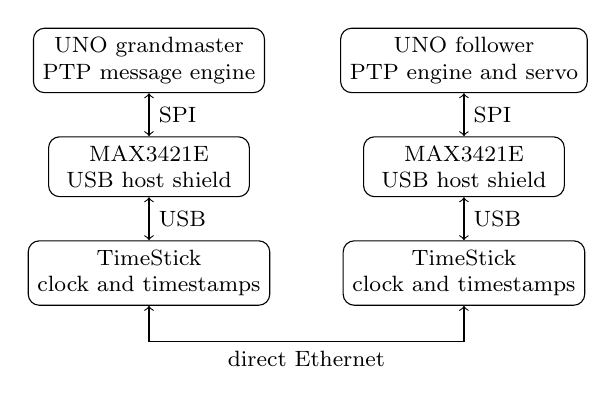
\begin{tikzpicture}[font=\footnotesize,box/.style={draw,rounded corners,align=center,minimum width=2.55cm,minimum height=.72cm}]
\node[box] (gm) at (0,0) {UNO grandmaster\\PTP message engine};
\node[box] (fl) at (4.0,0) {UNO follower\\PTP engine and servo};
\node[box] (gh) at (0,-1.35) {MAX3421E\\USB host shield};
\node[box] (fh) at (4.0,-1.35) {MAX3421E\\USB host shield};
\node[box] (gt) at (0,-2.7) {TimeStick\\clock and timestamps};
\node[box] (ft) at (4.0,-2.7) {TimeStick\\clock and timestamps};
\draw[<->] (gm)--node[right]{SPI}(gh);
\draw[<->] (fl)--node[right]{SPI}(fh);
\draw[<->] (gh)--node[right]{USB}(gt);
\draw[<->] (fh)--node[right]{USB}(ft);
\draw[<->] (gt.south)--++(0,-.45)--node[below]{direct Ethernet}++(4,0)--(ft.south);
\end{tikzpicture}
\caption{Timing hardware and control partition. Packet timestamps originate in the TimeSticks. The host computer, omitted here, only uploads firmware and records serial output.}
\label{fig:architecture}
\end{figure}

\subsection{Protocol and clock arithmetic}
The experiment uses Ethernet PTPv2, EtherType \texttt{0x88F7}, domain 42, two-step Sync, and end-to-end delay measurement at approximately one accepted exchange per second. Let $t_1$ denote grandmaster Sync transmission, $t_2$ follower Sync reception, $t_3$ follower Delay\_Req transmission, and $t_4$ grandmaster Delay\_Req reception. Define the corrected directional intervals as
\begin{equation}
 a=(t_2-t_1)-c_f,\qquad b=(t_4-t_3)-c_r,
\end{equation}
where $c_f$ and $c_r$ are the applicable correction fields expressed in nanoseconds. Under the symmetric-delay assumption, the estimates are
\begin{equation}
 \hat e=\frac{a-b}{2},\qquad \hat d=\frac{a+b}{2}.
 \label{eq:measurement}
\end{equation}
Here $\hat e$ is follower-minus-grandmaster phase. For forward and reverse delays $d_f$ and $d_r$, respectively, the offset estimate contains a bias $(d_f-d_r)/2$. Driving $\hat e$ toward zero cannot identify or remove this asymmetry.

The implementation matches domain, peer identity, and sequence identifiers, rejects incomplete or stale exchanges, and clears pending state after clock steps and link loss. Seconds and nanoseconds are stored separately. The supported diagnostic epoch uses 32-bit seconds; wire timestamps with nonzero upper seconds bits are rejected. Signed 64-bit differences avoid converting the entire wire epoch into a single nanosecond count. Correction fields retain their signed fractional representation until exchange arithmetic, whose output is integer nanoseconds.

The tested transmit-timestamp endpoint supplies a 131-byte report assembled from USB packets of 64, 64, and 3 bytes. Receive aggregates are bounds-checked; data beyond the configured storage are drained rather than written past the buffer. Plausibility checks reject path estimates outside $[-1000,10^6]$ ns. These are defensive bounds for the experiment, not a characterization of physical delay uncertainty.

\subsection{Acquisition, actuation, and observability}
Frequency corrections update the peripheral clock addend through USB control transfers. Large offsets use an absolute clock set, which has USB latency and therefore leaves a residual that the frequency servo must remove. R4 steps when the first accepted offset exceeds 1 ms in magnitude; later exchanges retain a 500 ms threshold. R3 retains 500 ms for both. The smaller initial threshold addresses Arduino uploads that do not reset the two peripheral clocks to a common phase.

Each controller is bounded to $\pm500{,}000$ ppb. Serial output at 115200 baud reports the unfiltered four-timestamp offset, frequency command, path estimate, and exchange counters. The status \texttt{s3} requires eight consecutive accepted offsets within $\pm1000$ ns. It is a state-machine indication, not an independent accuracy measurement. PPS outputs were enabled with register readback. The original five-servo R4 campaign used internal estimates; a separate fixed-PI PPS follow-up is reported in Section~\ref{sec:pps}.

\section{Clock Controllers}
All five controllers use the same protocol measurements and hardware actuator. With phase in nanoseconds and frequency in ppb, one ppb is numerically one nanosecond per second. Positive applied command $u$ increases follower clock frequency. Ignoring noise and actuation latency, the controlled phase evolves approximately as
\begin{equation}
 e_{k+1}=e_k+(f_k+u_k)\Delta t_k,
 \label{eq:plant}
\end{equation}
where $f_k$ is intrinsic follower frequency error relative to the grandmaster. Model-based controllers account for the previous command, rather than interpreting controlled phase slopes as intrinsic drift.

\subsection{Fixed and gain-scheduled PI}
The fixed PI baseline targets the one-second update period. In its unsaturated regime it forms
\begin{equation}
 I_k=I_{k-1}-\hat e_k/20,\qquad
 u_k=I_k-\hat e_k/2.
\end{equation}
The source uses integer division, an integral bound of $\pm200{,}000$ ppb, and conditional integration to prevent windup at the output limit. Quantization of the integral increment is relevant near zero offset.

The adaptive option schedules three $(K_p,K_i)$ pairs: $(0.25,0.016)$, $(0.5,0.05)$, and $(0.75,0.125)$, with units $\mathrm{s}^{-1}$ and $\mathrm{s}^{-2}$. It begins in the fastest setting and returns there for offsets beyond $\pm1000$ ns. Within that band, non-overlapping 16-sample windows evaluate offset magnitude, signed bias, and sign reversals. Persistent bias raises the gain one level. Small residuals or oscillatory sign changes can lower it, with two qualifying windows required for a reduction. This is a bounded heuristic, not an optimization procedure or an identified noise model.

The adaptive implementation also retains fractional integral precision and uses elapsed Sync time. Gain transitions compensate the integral to reduce command discontinuity. Consequently, comparing it with fixed PI evaluates several implementation differences together; it does not isolate gain scheduling alone.

\subsection{Linear regression}
The regression controller stores eight accepted observations. It reconstructs uncontrolled phase by subtracting accumulated applied corrections,
\begin{equation}
 y_k=\hat e_k-\sum_{j<k}u_j\Delta t_j,
\end{equation}
and fits an ordinary least-squares line using centered integer arithmetic. The fitted slope estimates intrinsic drift. Fitted current phase is reconstructed by adding the correction integral back; the command cancels drift and removes that phase over four seconds. At least four points are required before the first fit. History is discarded after invalid exchanges or unacceptable intervals. This fixed eight-point controller does not implement LinuxPTP's adaptive regression window.

\subsection{Kalman controller}
The Kalman state is $x=[e\ f]^T$. Prediction uses
\begin{equation}
 x^-_{k+1}=\begin{bmatrix}1&\Delta t_k\\0&1\end{bmatrix}x_k
 +\begin{bmatrix}\Delta t_k\\0\end{bmatrix}u_k,
 \qquad H=\begin{bmatrix}1&0\end{bmatrix}.
\end{equation}
The process covariance is
\begin{equation}
 Q=\begin{bmatrix}
 q_f\Delta t^3/3+q_p\Delta t&q_f\Delta t^2/2\\
 q_f\Delta t^2/2&q_f\Delta t
 \end{bmatrix},
\end{equation}
with $q_f=4\unit{ppb^2/s}$, $q_p=1\unit{ns^2/s}$, and measurement variance $R=100\unit{ns^2}$. Initial phase and frequency variances are $100\unit{ns^2}$ and $10^6\unit{ppb^2}$. These are fixed provisional settings. The command is $u=\clip(-\hat f-\hat e/(4\unit{s}))$, where the phase term denotes division by four seconds. A Joseph-form covariance update and bounded state checks address numerical fragility. Only residual phase, not an absolute epoch, is represented in single precision. R4 hardware floating-point instructions accelerate this existing arithmetic.

\subsection{Hybrid PLL/FLL}
The hybrid controller estimates intrinsic frequency over eight accepted intervals:
\begin{equation}
 \tilde f=\frac{\hat e_k-\hat e_a-\sum_{j=a}^{k-1}u_j\Delta t_j}
 {\sum_{j=a}^{k-1}\Delta t_j}.
\end{equation}
The first window initializes frequency; later windows update it with gain $1/2$. Each accepted observation also contributes a proportional phase correction with a four-second removal time. Only the endpoint phases enter the frequency estimate, while every applied command enters its integral. The implementation uses fixed-point arithmetic without a sample ring buffer. Reduced noise sensitivity competes with lag in tracking oscillator changes.

\section{Experimental Method}
The R4 measurements were collected on October 15, 2026, from 00:43:19 to 01:24:49 UTC. The same two TimeSticks and direct cable were used throughout. The grandmaster was uploaded once; the follower was uploaded successively with PI, regression, adaptive PI, Kalman, and PLL/FLL firmware for 300-second captures, then PI again for a 900-second capture. Grandmaster serial output was recorded continuously. This is a sequential feasibility campaign, without randomized order, controlled temperature, or identical initial phase.

Each short capture contains 288 accepted exchanges; the longer capture contains 888. Duration includes initialization, explaining why sample counts are smaller than nominal duration at 1 Hz. Every follower record has one boot marker, the expected platform and servo identifiers, and a matching log hash. Firmware hashes identify the uploaded images. Across all six records, accepted sample numbering is continuous. Reported timeout, missing-receive-timestamp, and discard counters remain zero, with no path rejections in the final campaign.

The master has one MCU boot but six link-down/reinitialization events associated with follower uploads. Its role counters restart at those boundaries. The records therefore must not be treated as one uninterrupted master-clock experiment. Earlier interrupted attempts, including initialization failures and host sleep gaps, remain archived separately and are not included in the final statistics.

A common cutoff of 120 seconds after the first accepted exchange defines the analysis window. All later samples are retained regardless of servo state or magnitude. For $N$ retained offsets,
\begin{equation}
 e_{\mathrm{RMS}}=\sqrt{\frac{1}{N}\sum_{k=1}^{N}\hat e_k^2},\qquad
 \sigma_e=\sqrt{\frac{1}{N}\sum_{k=1}^{N}(\hat e_k-\bar e)^2}.
\end{equation}
No smoothing or filter-state substitution is applied to these statistics. Settling is the beginning of the final uninterrupted suffix inside a stated band, provided that suffix lasts at least 30 seconds. This retrospective definition describes the finite record only. It differs from the eight-sample \texttt{s3} indication.

Servo profiling brackets filter arithmetic. Periodically emitted last-update durations provide a sampled median, not a median over all invocations. The separate USB polling duration includes parsing, callbacks, and clock and serial I/O; it is not a pure USB transfer time or a processor-utilization measurement. Trial images use Arm GNU Toolchain 13.3.Rel1, Arduino R4 core 1.6.0, and USB Host Shield Library 2.0 version 1.7.0.

\section{Results}
\subsection{Resource feasibility}
Table~\ref{tab:memory} reports the archived compile matrix for the same source generation. All five followers fit the R3 flash limit of 32,256 bytes. The Kalman build leaves only 118 bytes of that program budget. Static allocation does not include runtime stack usage, whose high-water mark was not measured. R4 increases available memory and supports the larger aggregate buffer while retaining the controller equations.

\begin{table}[t]
\centering\caption{Compiled follower resource use in bytes}
\label{tab:memory}
\begin{tabular}{lrrrr}\toprule
&\multicolumn{2}{c}{UNO R3}&\multicolumn{2}{c}{UNO R4}\\
Servo&Flash&Static RAM&Flash&Static RAM\\\midrule
PI&29,152&995&64,084&9,080\\
Regression&31,546&1,105&64,656&9,224\\
Adaptive PI&30,996&1,017&64,996&9,100\\
Kalman&32,138&1,017&64,612&9,100\\
PLL/FLL&29,984&1,016&64,424&9,104\\\bottomrule
\end{tabular}
\par\smallskip\footnotesize R3: AVR GCC 15.2.0, core 1.8.8. R4: Arm GCC 13.3.Rel1, core 1.6.0. Static RAM is not total runtime memory.
\end{table}

\subsection{Post-acquisition behavior}
Each short trial retains 167 samples spanning 166 seconds, all in \texttt{s3}. Table~\ref{tab:results} reports raw-offset statistics and arithmetic timing. Adaptive PI has the lowest RMS in this sequence. However, the measurements are not independent replicates under matched oscillator conditions, and the gain scheduler changes integral precision as well as gains. These data do not establish general superiority of one controller.

\begin{table}[t]
\centering\caption{R4 post-cutoff results, 167 offsets per servo}
\label{tab:results}
\begin{tabular}{lrrrr}\toprule
&\multicolumn{2}{c}{Offset (ns)}&\multicolumn{2}{c}{Update ($\mu$s)}\\
Servo&RMS&Min / max&Median&Peak\\\midrule
PI&41.01&$-110$ / $20$&6&9\\
Regression&33.93&$-105$ / $50$&22&25\\
Adaptive PI&16.35&$-50$ / $30$&12&15\\
Kalman&40.77&$-105$ / $65$&9&11\\
PLL/FLL&83.83&$-195$ / $140$&7&11\\\bottomrule
\end{tabular}
\par\smallskip\footnotesize Median is from sampled last-update telemetry; peak is the reported window maximum. Offset is an internal estimate.
\end{table}

% BEGIN_STEADY_FIGURE
\begin{figure}[t]
\centering
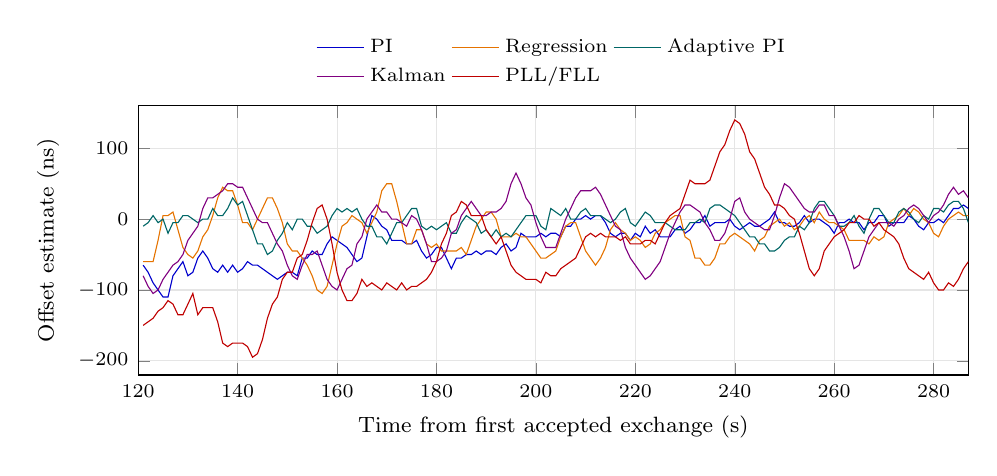
\begin{tikzpicture}
\begin{axis}[width=\columnwidth,height=5.0cm,scale only axis=false,tick label style={font=\scriptsize},label style={font=\footnotesize},grid=major,grid style={gray!20},xlabel={Time from first accepted exchange (s)},legend style={font=\scriptsize,draw=none,at={(0.5,1.03)},anchor=south,legend columns=3},legend cell align=left,xmin=120,xmax=287,ymin=-220,ymax=160,ylabel={Offset estimate (ns)}]
\addplot+[no marks,thin,color=blue!80!black] coordinates {
(120.993,-65)
(121.993,-75)
(122.993,-90)
(123.993,-100)
(124.993,-110)
(125.994,-110)
(126.993,-80)
(127.993,-70)
(128.993,-60)
(129.994,-80)
(130.993,-75)
(131.994,-55)
(132.993,-45)
(133.993,-55)
(134.993,-70)
(135.993,-75)
(136.993,-65)
(137.993,-75)
(138.993,-65)
(139.993,-75)
(140.993,-70)
(141.993,-60)
(142.993,-65)
(143.993,-65)
(144.993,-70)
(145.993,-75)
(146.993,-80)
(147.993,-85)
(148.993,-80)
(149.993,-75)
(150.993,-75)
(151.994,-80)
(152.993,-55)
(153.994,-55)
(154.993,-45)
(155.993,-50)
(156.993,-50)
(157.993,-35)
(158.993,-25)
(159.993,-30)
(160.993,-35)
(161.993,-40)
(162.993,-50)
(163.993,-60)
(164.993,-55)
(165.993,-25)
(166.993,5)
(167.993,0)
(168.993,-10)
(169.994,-15)
(170.993,-30)
(171.993,-30)
(172.993,-30)
(173.993,-35)
(174.993,-35)
(175.993,-30)
(176.993,-45)
(177.993,-55)
(178.993,-50)
(179.994,-40)
(180.993,-40)
(181.993,-55)
(182.993,-70)
(183.993,-55)
(184.993,-55)
(185.993,-50)
(186.993,-50)
(187.994,-45)
(188.993,-50)
(189.994,-45)
(190.993,-45)
(191.993,-50)
(192.993,-40)
(193.994,-35)
(194.993,-45)
(195.994,-40)
(196.993,-20)
(197.993,-25)
(198.993,-25)
(199.993,-25)
(200.993,-20)
(201.993,-25)
(202.993,-20)
(203.993,-20)
(204.993,-25)
(205.993,-10)
(206.993,-10)
(207.993,0)
(208.993,0)
(209.994,5)
(210.993,0)
(211.993,5)
(212.993,5)
(213.993,-5)
(214.993,-20)
(215.994,-25)
(216.993,-20)
(217.993,-20)
(218.993,-30)
(219.994,-20)
(220.993,-25)
(221.994,-10)
(222.993,-20)
(223.993,-15)
(224.993,-25)
(225.993,-25)
(226.993,-25)
(227.993,-15)
(228.993,-10)
(229.993,-20)
(230.993,-15)
(231.993,-5)
(232.993,-5)
(233.993,5)
(234.993,-10)
(235.993,-5)
(236.993,-5)
(237.993,-5)
(238.993,0)
(239.993,-10)
(240.993,-15)
(241.994,-10)
(242.993,-5)
(243.993,-10)
(244.993,-10)
(245.993,-5)
(246.993,0)
(247.993,10)
(248.993,-5)
(249.993,-5)
(250.993,-10)
(251.993,-10)
(252.993,-5)
(253.994,5)
(254.993,-5)
(255.993,0)
(256.993,0)
(257.994,-5)
(258.993,-10)
(259.994,-20)
(260.993,-5)
(261.993,-5)
(262.993,0)
(263.993,-5)
(264.993,-5)
(265.993,-15)
(266.993,-5)
(267.994,-5)
(268.993,5)
(269.993,5)
(270.993,-10)
(271.993,-5)
(272.993,-5)
(273.994,-5)
(274.993,5)
(275.993,0)
(276.993,-10)
(277.993,-15)
(278.993,-5)
(279.993,-5)
(280.993,0)
(281.993,-5)
(282.993,5)
(283.994,15)
(284.993,15)
(285.994,20)
(286.993,15)
};
\addplot+[no marks,thin,color=orange!90!black] coordinates {
(120.993,-60)
(121.993,-60)
(122.993,-60)
(123.993,-30)
(124.993,5)
(125.993,5)
(126.992,10)
(127.993,-15)
(128.993,-40)
(129.993,-50)
(130.993,-55)
(131.993,-45)
(132.993,-25)
(133.993,-15)
(134.992,5)
(135.993,30)
(136.993,45)
(137.993,40)
(138.993,40)
(139.993,20)
(140.992,-5)
(141.993,-5)
(142.993,-15)
(143.993,0)
(144.993,15)
(145.993,30)
(146.992,30)
(147.993,15)
(148.993,-5)
(149.993,-35)
(150.993,-45)
(151.993,-45)
(152.992,-55)
(153.993,-65)
(154.993,-80)
(155.993,-100)
(156.993,-105)
(157.993,-95)
(158.993,-65)
(159.993,-35)
(160.993,-10)
(161.993,-5)
(162.993,5)
(163.993,0)
(164.993,-5)
(165.993,-20)
(166.992,-5)
(167.993,10)
(168.993,40)
(169.993,50)
(170.993,50)
(171.993,25)
(172.992,-5)
(173.993,-35)
(174.993,-35)
(175.993,-15)
(176.993,-15)
(177.993,-35)
(178.993,-40)
(179.993,-35)
(180.993,-45)
(181.993,-45)
(182.993,-45)
(183.993,-45)
(184.993,-40)
(185.993,-50)
(186.993,-30)
(187.993,-10)
(188.993,0)
(189.993,10)
(190.993,10)
(191.993,0)
(192.993,-25)
(193.993,-25)
(194.993,-25)
(195.993,-20)
(196.993,-25)
(197.993,-25)
(198.993,-35)
(199.993,-45)
(200.993,-55)
(201.993,-55)
(202.993,-50)
(203.993,-45)
(204.992,-25)
(205.993,-10)
(206.993,-5)
(207.993,-5)
(208.993,-25)
(209.993,-45)
(210.992,-55)
(211.993,-65)
(212.993,-55)
(213.993,-40)
(214.993,-15)
(215.993,-5)
(216.993,-15)
(217.993,-20)
(218.993,-30)
(219.993,-25)
(220.993,-30)
(221.993,-40)
(222.993,-35)
(223.993,-20)
(224.992,-15)
(225.993,-5)
(226.993,0)
(227.993,5)
(228.993,5)
(229.993,-25)
(230.992,-30)
(231.993,-55)
(232.993,-55)
(233.993,-65)
(234.992,-65)
(235.993,-55)
(236.993,-35)
(237.993,-35)
(238.993,-25)
(239.993,-20)
(240.993,-25)
(241.993,-30)
(242.992,-35)
(243.993,-45)
(244.993,-30)
(245.993,-25)
(246.993,-10)
(247.993,-5)
(248.993,0)
(249.993,-10)
(250.992,-5)
(251.993,-15)
(252.993,-10)
(253.993,0)
(254.993,5)
(255.993,-5)
(256.993,10)
(257.994,0)
(258.993,-5)
(259.993,-5)
(260.993,-10)
(261.993,-15)
(262.992,-30)
(263.993,-30)
(264.993,-30)
(265.993,-30)
(266.993,-35)
(267.993,-25)
(268.993,-30)
(269.994,-25)
(270.992,-5)
(271.993,0)
(272.993,5)
(273.993,15)
(274.993,5)
(275.993,15)
(276.993,10)
(277.993,0)
(278.993,-5)
(279.993,-20)
(280.993,-25)
(281.993,-10)
(282.993,0)
(283.994,5)
(284.993,10)
(285.993,5)
(286.993,5)
};
\addplot+[no marks,thin,color=teal!80!black] coordinates {
(120.996,-10)
(121.995,-5)
(122.996,5)
(123.996,-5)
(124.996,0)
(125.996,-20)
(126.996,-5)
(127.995,-5)
(128.996,5)
(129.996,5)
(130.996,0)
(131.996,-5)
(132.996,0)
(133.996,0)
(134.996,15)
(135.995,5)
(136.996,5)
(137.996,15)
(138.996,30)
(139.996,20)
(140.996,25)
(141.996,5)
(142.996,-15)
(143.996,-35)
(144.996,-35)
(145.996,-50)
(146.996,-45)
(147.995,-30)
(148.996,-20)
(149.996,-5)
(150.996,-15)
(151.996,0)
(152.996,0)
(153.995,-10)
(154.996,-10)
(155.997,-20)
(156.996,-15)
(157.996,-10)
(158.996,5)
(159.996,15)
(160.996,10)
(161.996,15)
(162.996,10)
(163.996,15)
(164.996,0)
(165.996,-10)
(166.996,-10)
(167.995,-25)
(168.996,-25)
(169.996,-35)
(170.996,-20)
(171.996,-5)
(172.996,-5)
(173.996,5)
(174.996,15)
(175.996,15)
(176.996,-10)
(177.996,-15)
(178.996,-10)
(179.996,-15)
(180.996,-10)
(181.996,-5)
(182.996,-20)
(183.996,-20)
(184.996,-5)
(185.996,5)
(186.996,0)
(187.995,-5)
(188.996,-20)
(189.996,-15)
(190.996,-25)
(191.996,-15)
(192.996,-25)
(193.996,-20)
(194.996,-25)
(195.996,-15)
(196.996,-5)
(197.996,5)
(198.996,5)
(199.996,5)
(200.996,-10)
(201.996,-15)
(202.996,15)
(203.996,10)
(204.996,5)
(205.995,15)
(206.996,0)
(207.996,0)
(208.996,10)
(209.996,15)
(210.996,5)
(211.996,5)
(212.996,5)
(213.996,0)
(214.996,-5)
(215.996,0)
(216.996,10)
(217.995,15)
(218.996,-5)
(219.995,-10)
(220.996,0)
(221.996,10)
(222.996,5)
(223.996,-5)
(224.996,-5)
(225.996,-5)
(226.996,-10)
(227.996,-15)
(228.996,-15)
(229.996,-15)
(230.996,-5)
(231.995,-5)
(232.996,0)
(233.996,-5)
(234.996,15)
(235.996,20)
(236.996,20)
(237.995,15)
(238.996,10)
(239.996,5)
(240.996,-5)
(241.996,-15)
(242.996,-25)
(243.996,-25)
(244.996,-35)
(245.996,-35)
(246.996,-45)
(247.996,-45)
(248.996,-40)
(249.996,-30)
(250.996,-25)
(251.996,-25)
(252.996,-10)
(253.996,-15)
(254.996,-5)
(255.996,15)
(256.996,25)
(257.996,25)
(258.996,15)
(259.996,5)
(260.996,-10)
(261.996,-10)
(262.996,-5)
(263.996,5)
(264.996,-10)
(265.996,-20)
(266.996,0)
(267.996,15)
(268.996,15)
(269.995,5)
(270.996,-5)
(271.996,-5)
(272.996,10)
(273.996,15)
(274.996,10)
(275.996,0)
(276.996,-5)
(277.996,5)
(278.996,0)
(279.996,15)
(280.996,15)
(281.996,10)
(282.996,20)
(283.996,25)
(284.996,25)
(285.996,15)
(286.996,-5)
};
\addplot+[no marks,thin,color=violet] coordinates {
(120.994,-80)
(121.994,-95)
(122.994,-105)
(123.994,-100)
(124.994,-85)
(125.994,-75)
(126.994,-65)
(127.994,-60)
(128.994,-50)
(129.994,-30)
(130.994,-20)
(131.994,-10)
(132.994,15)
(133.994,30)
(134.994,30)
(135.994,35)
(136.994,40)
(137.994,50)
(138.994,50)
(139.994,45)
(140.994,45)
(141.994,30)
(142.994,15)
(143.994,0)
(144.994,-5)
(145.994,-5)
(146.994,-20)
(147.994,-35)
(148.994,-45)
(149.994,-65)
(150.994,-80)
(151.994,-85)
(152.994,-65)
(153.994,-50)
(154.994,-50)
(155.994,-45)
(156.994,-65)
(157.994,-85)
(158.994,-95)
(159.994,-100)
(160.994,-85)
(161.994,-70)
(162.994,-65)
(163.994,-35)
(164.994,-25)
(165.994,0)
(166.994,10)
(167.994,20)
(168.995,10)
(169.994,10)
(170.994,0)
(171.994,0)
(172.994,-5)
(173.994,-10)
(174.994,5)
(175.994,0)
(176.994,-15)
(177.994,-35)
(178.994,-60)
(179.994,-60)
(180.995,-55)
(181.994,-45)
(182.994,-20)
(183.994,-15)
(184.994,5)
(185.994,15)
(186.994,25)
(187.994,15)
(188.994,5)
(189.994,5)
(190.994,10)
(191.994,10)
(192.994,15)
(193.994,25)
(194.994,50)
(195.994,65)
(196.994,50)
(197.994,30)
(198.994,20)
(199.994,-5)
(200.994,-25)
(201.994,-40)
(202.994,-40)
(203.994,-40)
(204.994,-20)
(205.994,0)
(206.995,15)
(207.994,30)
(208.994,40)
(209.994,40)
(210.994,40)
(211.994,45)
(212.994,35)
(213.994,20)
(214.994,5)
(215.994,-10)
(216.994,-15)
(217.994,-40)
(218.994,-55)
(219.994,-65)
(220.994,-75)
(221.994,-85)
(222.994,-80)
(223.994,-70)
(224.994,-60)
(225.994,-40)
(226.994,-20)
(227.994,-5)
(228.994,10)
(229.994,20)
(230.994,20)
(231.994,15)
(232.994,10)
(233.994,-5)
(234.994,-15)
(235.994,-30)
(236.994,-30)
(237.994,-20)
(238.994,0)
(239.994,25)
(240.994,30)
(241.994,10)
(242.994,0)
(243.994,-5)
(244.994,-10)
(245.994,-15)
(246.994,-15)
(247.994,5)
(248.994,30)
(249.994,50)
(250.994,45)
(251.994,35)
(252.994,25)
(253.994,15)
(254.994,10)
(255.994,10)
(256.994,20)
(257.994,20)
(258.994,5)
(259.994,5)
(260.994,-10)
(261.994,-25)
(262.994,-45)
(263.994,-70)
(264.994,-65)
(265.994,-45)
(266.994,-25)
(267.994,-15)
(268.994,-5)
(269.994,-5)
(270.994,-5)
(271.994,-10)
(272.994,0)
(273.994,5)
(274.994,15)
(275.994,20)
(276.994,15)
(277.994,5)
(278.994,-5)
(279.994,5)
(280.994,10)
(281.994,20)
(282.994,35)
(283.994,45)
(284.994,35)
(285.994,40)
(286.994,30)
};
\addplot+[no marks,thin,color=red!75!black] coordinates {
(120.994,-150)
(121.994,-145)
(122.994,-140)
(123.994,-130)
(124.994,-125)
(125.994,-115)
(126.994,-120)
(127.994,-135)
(128.994,-135)
(129.994,-120)
(130.994,-105)
(131.994,-135)
(132.994,-125)
(133.994,-125)
(134.994,-125)
(135.993,-145)
(136.994,-175)
(137.994,-180)
(138.994,-175)
(139.994,-175)
(140.994,-175)
(141.994,-180)
(142.994,-195)
(143.994,-190)
(144.994,-170)
(145.994,-140)
(146.994,-120)
(147.994,-110)
(148.994,-85)
(149.994,-75)
(150.994,-75)
(151.994,-55)
(152.994,-50)
(153.994,-30)
(154.994,-5)
(155.994,15)
(156.994,20)
(157.994,0)
(158.994,-35)
(159.994,-75)
(160.994,-100)
(161.994,-115)
(162.994,-115)
(163.994,-105)
(164.994,-85)
(165.994,-95)
(166.994,-90)
(167.994,-95)
(168.994,-100)
(169.994,-90)
(170.994,-95)
(171.994,-100)
(172.994,-90)
(173.994,-100)
(174.994,-95)
(175.994,-95)
(176.994,-90)
(177.994,-85)
(178.994,-75)
(179.994,-60)
(180.994,-35)
(181.994,-20)
(182.994,5)
(183.993,10)
(184.994,25)
(185.994,20)
(186.994,5)
(187.994,5)
(188.994,5)
(189.994,-15)
(190.994,-25)
(191.994,-35)
(192.994,-25)
(193.994,-45)
(194.994,-65)
(195.994,-75)
(196.994,-80)
(197.993,-85)
(198.994,-85)
(199.994,-85)
(200.994,-90)
(201.994,-75)
(202.994,-80)
(203.994,-80)
(204.994,-70)
(205.994,-65)
(206.994,-60)
(207.994,-55)
(208.994,-40)
(209.993,-25)
(210.994,-20)
(211.993,-25)
(212.994,-20)
(213.993,-25)
(214.994,-25)
(215.994,-25)
(216.994,-30)
(217.994,-25)
(218.994,-35)
(219.994,-35)
(220.994,-35)
(221.994,-30)
(222.994,-30)
(223.994,-35)
(224.994,-20)
(225.993,-5)
(226.994,5)
(227.994,10)
(228.994,15)
(229.994,35)
(230.994,55)
(231.994,50)
(232.994,50)
(233.994,50)
(234.994,55)
(235.994,75)
(236.994,95)
(237.993,105)
(238.994,125)
(239.994,140)
(240.994,135)
(241.994,120)
(242.994,95)
(243.994,85)
(244.994,65)
(245.994,45)
(246.994,35)
(247.994,20)
(248.994,20)
(249.994,15)
(250.994,5)
(251.994,0)
(252.994,-20)
(253.994,-45)
(254.994,-70)
(255.994,-80)
(256.994,-70)
(257.994,-45)
(258.994,-35)
(259.994,-25)
(260.994,-20)
(261.994,-15)
(262.994,-5)
(263.994,-5)
(264.994,5)
(265.994,0)
(266.994,0)
(267.994,-10)
(268.994,-5)
(269.994,-15)
(270.994,-20)
(271.994,-25)
(272.994,-35)
(273.993,-55)
(274.994,-70)
(275.994,-75)
(276.994,-80)
(277.994,-85)
(278.994,-75)
(279.994,-90)
(280.994,-100)
(281.994,-100)
(282.994,-90)
(283.994,-95)
(284.994,-85)
(285.994,-70)
(286.994,-60)
};
\legend{PI,Regression,Adaptive PI,Kalman,PLL/FLL}
\end{axis}
\end{tikzpicture}
\caption{R4 raw offset estimates after the common 120-second cutoff. Every retained sample is plotted. Traces are separate sequential trials, not simultaneous measurements.}
\label{fig:steady}
\end{figure}
% END_STEADY_FIGURE

The Kalman sampled median is 9 $\mu$s, compared with 22 $\mu$s for the integer regression. This is an R4 implementation result, not a measured speedup relative to R3. The largest steady-window arithmetic peak is 25 $\mu$s, small relative to the one-second exchange period. USB polling sections reach approximately 3.1--3.8 ms and include work beyond the controller itself. The processor has arithmetic headroom at this rate, although worst-case execution time and overload behavior remain unmeasured.

\subsection{Startup transients}
Every short trial begins with a coarse step. Initial offsets range from approximately $-254$ to $-868$ ms. Table~\ref{tab:transient} gives settling times from the first accepted exchange. They are observed trajectories with different initial conditions, not controlled acquisition-speed comparisons. The adaptive PI, Kalman, and PLL/FLL starts fall below the old 500 ms threshold and therefore exercise the R4-specific first-exchange rule on hardware.

\begin{table}[t]
\centering\caption{Observed R4 acquisition times}
\label{tab:transient}
\begin{tabular}{lrrr}\toprule
&Initial offset&\multicolumn{2}{c}{Settling time (s)}\\
Servo&(ms)&$\pm1000$ ns&$\pm100$ ns\\\midrule
PI&$-861.929$&43.99&126.99\\
Regression&$-868.118$&28.99&157.99\\
Adaptive PI&$-330.405$&29.00&44.00\\
Kalman&$-254.350$&25.99&123.99\\
PLL/FLL&$-256.198$&28.99&242.99\\\bottomrule
\end{tabular}
\end{table}

% BEGIN_TRANSIENT_FIGURE
\begin{figure}[t]
\centering
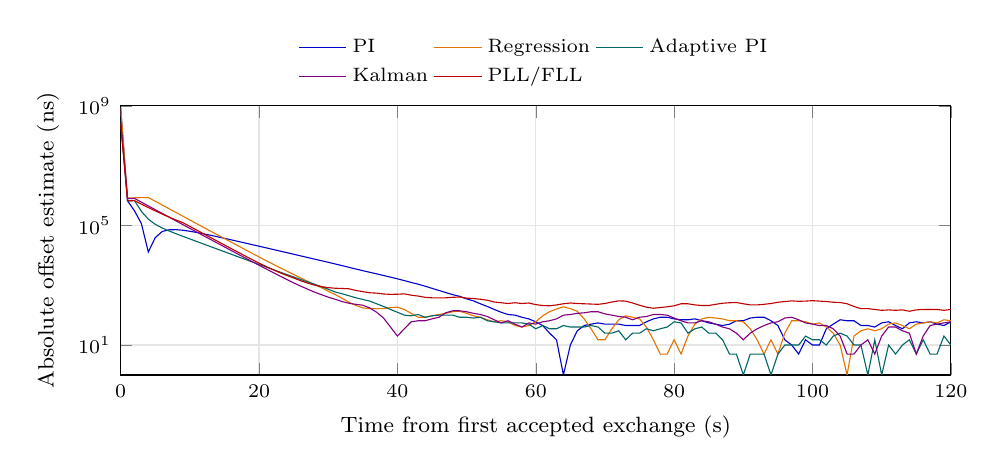
\begin{tikzpicture}
\begin{axis}[width=\columnwidth,height=5.0cm,scale only axis=false,tick label style={font=\scriptsize},label style={font=\footnotesize},grid=major,grid style={gray!20},xlabel={Time from first accepted exchange (s)},legend style={font=\scriptsize,draw=none,at={(0.5,1.03)},anchor=south,legend columns=3},legend cell align=left,xmin=0,xmax=120,ymode=log,ymin=1,ymax=1e9,ylabel={Absolute offset estimate (ns)}]
\addplot+[no marks,thin,color=blue!80!black] coordinates {
(0.0,861929180)
(0.993,662205)
(1.993,308640)
(2.993,115300)
(3.994,12930)
(4.993,38745)
(5.993,62595)
(6.993,71355)
(7.994,72150)
(8.993,68925)
(9.994,63860)
(10.993,58125)
(11.993,52350)
(12.993,46835)
(13.994,41735)
(14.993,37080)
(15.994,32885)
(16.993,29130)
(17.993,25795)
(18.993,22825)
(19.993,20200)
(20.993,17875)
(21.993,15785)
(22.993,13955)
(23.993,12320)
(24.993,10890)
(25.993,9615)
(26.993,8480)
(27.993,7495)
(28.993,6625)
(29.994,5850)
(30.993,5155)
(31.993,4530)
(32.993,3965)
(33.993,3490)
(34.993,3070)
(35.994,2710)
(36.993,2405)
(37.994,2115)
(38.993,1865)
(39.994,1640)
(40.993,1430)
(41.993,1240)
(42.993,1085)
(43.993,930)
(44.993,790)
(45.993,670)
(46.993,570)
(47.994,485)
(48.993,425)
(49.993,350)
(50.993,300)
(51.993,240)
(52.993,195)
(53.994,155)
(54.993,125)
(55.993,105)
(56.993,100)
(57.993,85)
(58.993,75)
(59.993,60)
(60.993,45)
(61.994,25)
(62.993,15)
(63.993,1)
(64.993,10)
(65.993,30)
(66.993,45)
(67.993,50)
(68.993,55)
(69.993,50)
(70.993,50)
(71.993,50)
(72.993,45)
(73.994,45)
(74.993,45)
(75.993,60)
(76.993,75)
(77.993,85)
(78.993,85)
(79.994,75)
(80.993,70)
(81.993,70)
(82.993,75)
(83.993,65)
(84.993,55)
(85.993,50)
(86.993,45)
(87.993,50)
(88.993,65)
(89.994,65)
(90.993,80)
(91.993,85)
(92.993,85)
(93.994,65)
(94.993,45)
(95.993,15)
(96.993,10)
(97.993,5)
(98.993,15)
(99.993,10)
(100.993,10)
(101.993,35)
(102.993,50)
(103.993,70)
(104.993,65)
(105.994,65)
(106.993,45)
(107.993,45)
(108.993,40)
(109.993,55)
(110.993,60)
(111.993,45)
(112.993,35)
(113.993,55)
(114.993,60)
(115.993,55)
(116.993,60)
(117.994,50)
(118.993,45)
(119.993,60)
};
\addplot+[no marks,thin,color=orange!90!black] coordinates {
(0.0,868118365)
(0.993,827635)
(1.993,837515)
(2.993,847415)
(3.993,857325)
(4.992,643685)
(5.993,482495)
(6.993,361715)
(7.993,271085)
(8.993,203195)
(9.993,152290)
(10.992,114195)
(11.993,85685)
(12.993,64410)
(13.993,48445)
(14.993,36460)
(15.993,27440)
(16.993,20660)
(17.993,15540)
(18.993,11720)
(19.993,8855)
(20.993,6710)
(21.993,5110)
(22.993,3905)
(23.993,2990)
(24.992,2285)
(25.993,1765)
(26.993,1365)
(27.993,1060)
(28.993,825)
(29.993,635)
(30.992,490)
(31.993,370)
(32.993,270)
(33.993,210)
(34.993,175)
(35.993,165)
(36.992,165)
(37.993,165)
(38.993,180)
(39.993,185)
(40.993,155)
(41.993,115)
(42.993,85)
(43.993,85)
(44.993,95)
(45.993,105)
(46.993,115)
(47.993,130)
(48.993,135)
(49.993,115)
(50.993,95)
(51.993,85)
(52.993,70)
(53.993,60)
(54.993,65)
(55.993,60)
(56.993,45)
(57.993,40)
(58.993,45)
(59.993,60)
(60.993,95)
(61.993,130)
(62.992,160)
(63.993,190)
(64.992,165)
(65.993,135)
(66.993,75)
(67.993,35)
(68.993,15)
(69.993,15)
(70.993,35)
(71.993,70)
(72.993,95)
(73.993,85)
(74.993,75)
(75.993,40)
(76.992,15)
(77.993,5)
(78.993,5)
(79.993,15)
(80.993,5)
(81.993,20)
(82.992,50)
(83.993,75)
(84.993,85)
(85.993,80)
(86.993,75)
(87.993,65)
(88.992,65)
(89.993,60)
(90.993,35)
(91.993,15)
(92.993,5)
(93.993,15)
(94.992,5)
(95.993,25)
(96.992,65)
(97.993,65)
(98.993,60)
(99.993,50)
(100.993,55)
(101.993,40)
(102.993,25)
(103.993,10)
(104.993,1)
(105.993,20)
(106.993,30)
(107.993,35)
(108.992,30)
(109.993,35)
(110.993,50)
(111.993,55)
(112.993,45)
(113.993,35)
(114.993,50)
(115.993,55)
(116.993,60)
(117.993,55)
(118.993,70)
(119.993,65)
};
\addplot+[no marks,thin,color=teal!80!black] coordinates {
(0.0,330404685)
(0.996,663960)
(1.996,673815)
(2.996,295020)
(3.996,161985)
(4.996,108810)
(5.995,82105)
(6.996,65200)
(7.996,52855)
(8.996,43175)
(9.996,35380)
(10.996,29030)
(11.995,23820)
(12.996,19560)
(13.995,16070)
(14.996,13205)
(15.996,10855)
(16.996,8910)
(17.996,7335)
(18.996,6030)
(19.995,4960)
(20.996,4095)
(21.996,3365)
(22.996,2770)
(23.996,2285)
(24.996,1895)
(25.995,1560)
(26.996,1295)
(27.996,1085)
(28.996,900)
(29.996,735)
(30.996,595)
(31.996,520)
(32.996,445)
(33.996,380)
(34.996,335)
(35.996,295)
(36.996,240)
(37.995,195)
(38.996,155)
(39.996,125)
(40.996,100)
(41.996,95)
(42.996,105)
(43.995,85)
(44.996,95)
(45.995,100)
(46.996,100)
(47.996,100)
(48.996,85)
(49.996,85)
(50.996,80)
(51.996,85)
(52.996,65)
(53.996,60)
(54.996,55)
(55.996,55)
(56.996,55)
(57.995,55)
(58.996,50)
(59.996,35)
(60.996,45)
(61.996,35)
(62.996,35)
(63.996,45)
(64.996,40)
(65.996,40)
(66.996,40)
(67.996,45)
(68.996,40)
(69.995,25)
(70.996,25)
(71.996,30)
(72.996,15)
(73.996,25)
(74.996,25)
(75.996,35)
(76.996,30)
(77.996,35)
(78.996,40)
(79.996,60)
(80.996,55)
(81.996,25)
(82.996,35)
(83.996,40)
(84.996,25)
(85.996,25)
(86.996,15)
(87.996,5)
(88.996,5)
(89.995,1)
(90.996,5)
(91.996,5)
(92.996,5)
(93.996,1)
(94.996,5)
(95.996,10)
(96.996,10)
(97.996,10)
(98.996,20)
(99.996,15)
(100.996,15)
(101.995,10)
(102.996,20)
(103.996,25)
(104.996,20)
(105.996,10)
(106.996,10)
(107.996,1)
(108.996,15)
(109.996,1)
(110.996,10)
(111.996,5)
(112.996,10)
(113.996,15)
(114.996,5)
(115.996,15)
(116.996,5)
(117.996,5)
(118.996,20)
(119.996,10)
};
\addplot+[no marks,thin,color=violet] coordinates {
(0.0,254350275)
(0.995,789775)
(1.994,799595)
(2.994,600205)
(3.994,449770)
(4.994,336935)
(5.994,252545)
(6.994,189255)
(7.994,141930)
(8.994,106440)
(9.994,79885)
(10.994,59975)
(11.994,45085)
(12.994,33895)
(13.994,25500)
(14.994,19180)
(15.994,14430)
(16.994,10870)
(17.994,8195)
(18.994,6185)
(19.994,4675)
(20.994,3545)
(21.994,2690)
(22.994,2050)
(23.994,1565)
(24.994,1200)
(25.994,940)
(26.994,745)
(27.994,590)
(28.994,485)
(29.994,400)
(30.994,340)
(31.994,285)
(32.994,250)
(33.994,230)
(34.994,215)
(35.994,175)
(36.994,125)
(37.994,80)
(38.994,40)
(39.994,20)
(40.994,35)
(41.994,60)
(42.994,65)
(43.994,65)
(44.994,75)
(45.993,85)
(46.994,120)
(47.994,140)
(48.994,140)
(49.994,130)
(50.994,115)
(51.994,105)
(52.994,90)
(53.994,70)
(54.994,55)
(55.994,65)
(56.994,50)
(57.994,40)
(58.994,55)
(59.994,50)
(60.994,60)
(61.994,65)
(62.994,75)
(63.994,100)
(64.994,105)
(65.994,115)
(66.994,120)
(67.994,130)
(68.994,130)
(69.994,110)
(70.994,100)
(71.994,90)
(72.994,85)
(73.994,70)
(74.994,85)
(75.994,90)
(76.994,105)
(77.994,105)
(78.994,100)
(79.994,80)
(80.994,65)
(81.994,55)
(82.994,55)
(83.994,65)
(84.994,60)
(85.994,50)
(86.994,40)
(87.994,35)
(88.994,25)
(89.994,15)
(90.995,25)
(91.994,35)
(92.994,45)
(93.994,55)
(94.994,60)
(95.994,80)
(96.994,85)
(97.994,70)
(98.994,55)
(99.994,50)
(100.994,45)
(101.994,45)
(102.994,35)
(103.994,20)
(104.994,5)
(105.994,5)
(106.994,10)
(107.994,15)
(108.994,5)
(109.994,20)
(110.994,40)
(111.994,40)
(112.994,30)
(113.994,25)
(114.994,5)
(115.994,20)
(116.995,45)
(117.994,50)
(118.994,55)
(119.994,60)
};
\addplot+[no marks,thin,color=red!75!black] coordinates {
(0.0,256197805)
(0.994,663925)
(1.993,673735)
(2.994,515450)
(3.994,396325)
(4.994,306935)
(5.994,239990)
(6.994,189750)
(7.994,152140)
(8.994,123920)
(9.994,92985)
(10.994,69745)
(11.994,52355)
(12.994,39315)
(13.994,29545)
(14.994,22235)
(15.994,16750)
(16.994,12640)
(17.994,9535)
(18.994,7230)
(19.994,5515)
(20.994,4265)
(21.994,3330)
(22.994,2640)
(23.994,2130)
(24.994,1755)
(25.994,1420)
(26.994,1185)
(27.994,1015)
(28.994,905)
(29.994,830)
(30.994,795)
(31.994,780)
(32.994,760)
(33.994,670)
(34.994,610)
(35.994,560)
(36.994,545)
(37.994,510)
(38.994,495)
(39.994,500)
(40.994,515)
(41.994,465)
(42.994,435)
(43.994,395)
(44.994,380)
(45.994,380)
(46.994,380)
(47.994,395)
(48.994,405)
(49.994,370)
(50.994,360)
(51.994,340)
(52.994,315)
(53.994,275)
(54.994,260)
(55.993,245)
(56.994,260)
(57.994,245)
(58.994,255)
(59.994,225)
(60.994,210)
(61.994,205)
(62.994,220)
(63.994,240)
(64.994,255)
(65.994,245)
(66.994,240)
(67.993,235)
(68.994,230)
(69.994,245)
(70.994,275)
(71.994,300)
(72.994,295)
(73.994,255)
(74.994,215)
(75.994,185)
(76.994,170)
(77.994,180)
(78.994,190)
(79.994,205)
(80.994,240)
(81.994,240)
(82.994,220)
(83.994,210)
(84.994,210)
(85.994,230)
(86.994,250)
(87.994,260)
(88.994,265)
(89.994,240)
(90.994,220)
(91.993,220)
(92.994,230)
(93.993,245)
(94.994,270)
(95.994,285)
(96.994,300)
(97.994,290)
(98.994,295)
(99.994,305)
(100.994,295)
(101.994,285)
(102.994,270)
(103.994,265)
(104.994,240)
(105.994,195)
(106.994,165)
(107.994,165)
(108.994,155)
(109.993,145)
(110.994,150)
(111.994,145)
(112.994,150)
(113.994,135)
(114.994,150)
(115.994,155)
(116.994,155)
(117.994,155)
(118.994,145)
(119.993,155)
};
\legend{PI,Regression,Adaptive PI,Kalman,PLL/FLL}
\end{axis}
\end{tikzpicture}
\caption{R4 startup trajectories, including initial coarse steps. Absolute values are used for the logarithmic axis; exact zero offsets are displayed at 1 ns only in this figure. Initial conditions differ between runs.}
\label{fig:transient}
\end{figure}
% END_TRANSIENT_FIGURE

\subsection{Longer PI record}
The 900-second PI capture retains 767 samples over 766 seconds after the same cutoff. RMS offset is 23.23 ns, mean offset is $-9.67$ ns, and population standard deviation is 21.12 ns. Offsets range from $-70$ to $+80$ ns. Mean path estimate is 733.82 ns, with a 725--745 ns range. All retained observations are in \texttt{s3}; the largest accepted-sample interval is 1.001 seconds. The sampled median PI update remains 6 $\mu$s, with a 7 $\mu$s peak.

The difference between the 41.01 ns short PI RMS and the 23.23 ns longer PI RMS is a reason to repeat experiments under controlled conditions. A single short window is not a stable basis for ranking servos. The longer record demonstrates continuity for about fifteen minutes including startup, not stability over hours, days, or temperature changes.

% BEGIN_LONG_FIGURE
\begin{figure}[t]
\centering
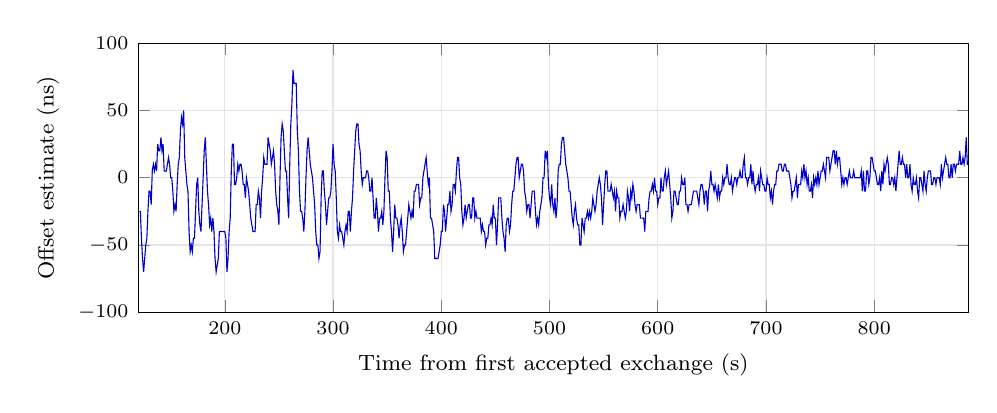
\begin{tikzpicture}
\begin{axis}[width=\columnwidth,height=5.0cm,scale only axis=false,tick label style={font=\scriptsize},label style={font=\footnotesize},grid=major,grid style={gray!20},xlabel={Time from first accepted exchange (s)},legend style={font=\scriptsize,draw=none,at={(0.5,1.03)},anchor=south,legend columns=3},legend cell align=left,xmin=120,xmax=887,ymin=-100,ymax=100,ylabel={Offset estimate (ns)}]
\addplot+[no marks,thin,color=blue!80!black] coordinates {
(120.993,-25)
(121.993,-25)
(122.994,-45)
(123.993,-60)
(124.993,-70)
(125.993,-60)
(126.994,-50)
(127.993,-45)
(128.994,-25)
(129.993,-10)
(130.994,-10)
(131.993,-20)
(132.994,5)
(133.993,10)
(134.994,5)
(135.993,10)
(136.993,5)
(137.993,25)
(138.994,20)
(139.993,20)
(140.994,30)
(141.993,20)
(142.994,25)
(143.993,5)
(144.994,5)
(145.993,5)
(146.993,10)
(147.993,15)
(148.994,10)
(149.993,0)
(150.994,0)
(151.993,-10)
(152.994,-25)
(153.993,-20)
(154.994,-25)
(155.993,-5)
(156.994,10)
(157.993,15)
(158.994,35)
(159.993,45)
(160.993,40)
(161.993,50)
(162.993,15)
(163.993,5)
(164.994,-5)
(165.993,-10)
(166.994,-40)
(167.993,-55)
(168.994,-50)
(169.993,-55)
(170.994,-45)
(171.993,-45)
(172.993,-25)
(173.993,-5)
(174.994,0)
(175.993,-25)
(176.993,-35)
(177.993,-40)
(178.994,-20)
(179.993,0)
(180.994,20)
(181.993,30)
(182.994,10)
(183.993,-10)
(184.994,-20)
(185.993,-35)
(186.994,-30)
(187.993,-40)
(188.993,-30)
(189.993,-40)
(190.994,-60)
(191.993,-70)
(192.994,-65)
(193.993,-60)
(194.994,-40)
(195.993,-40)
(196.994,-40)
(197.993,-40)
(198.994,-40)
(199.993,-40)
(200.994,-45)
(201.993,-70)
(202.994,-60)
(203.993,-40)
(204.994,-30)
(205.993,5)
(206.994,25)
(207.993,25)
(208.994,-5)
(209.993,-5)
(210.994,0)
(211.993,10)
(212.994,5)
(213.994,10)
(214.994,10)
(215.993,5)
(216.994,-5)
(217.993,-5)
(218.994,-15)
(219.993,0)
(220.994,-5)
(221.993,-10)
(222.994,-20)
(223.993,-30)
(224.994,-35)
(225.993,-40)
(226.994,-40)
(227.993,-40)
(228.994,-20)
(229.993,-20)
(230.994,-10)
(231.993,-15)
(232.994,-30)
(233.993,-10)
(234.994,0)
(235.993,15)
(236.994,10)
(237.993,10)
(238.994,10)
(239.994,30)
(240.993,25)
(241.993,20)
(242.994,10)
(243.993,15)
(244.994,20)
(245.993,10)
(246.994,-10)
(247.993,-20)
(248.994,-25)
(249.993,-35)
(250.993,0)
(251.993,30)
(252.994,40)
(253.993,35)
(254.994,20)
(255.993,5)
(256.994,5)
(257.993,-15)
(258.994,-30)
(259.993,10)
(260.994,40)
(261.993,55)
(262.993,80)
(263.993,70)
(264.994,70)
(265.993,70)
(266.994,35)
(267.993,20)
(268.994,-10)
(269.993,-25)
(270.994,-25)
(271.993,-30)
(272.994,-40)
(273.993,-25)
(274.994,0)
(275.993,20)
(276.993,30)
(277.994,20)
(278.994,10)
(279.993,5)
(280.994,0)
(281.993,-10)
(282.994,-20)
(283.993,-40)
(284.994,-50)
(285.993,-50)
(286.994,-60)
(287.993,-55)
(288.994,-15)
(289.993,5)
(290.994,5)
(291.993,-10)
(292.994,-20)
(293.993,-35)
(294.994,-25)
(295.993,-15)
(296.994,-15)
(297.993,-10)
(298.994,5)
(299.993,25)
(300.994,10)
(301.993,5)
(302.994,-15)
(303.994,-40)
(304.993,-45)
(305.993,-35)
(306.993,-40)
(307.993,-40)
(308.993,-45)
(309.993,-50)
(310.993,-40)
(311.993,-35)
(312.993,-40)
(313.993,-25)
(314.993,-25)
(315.993,-40)
(316.994,-25)
(317.993,-15)
(318.993,5)
(319.993,20)
(320.993,35)
(321.993,40)
(322.993,40)
(323.993,25)
(324.993,20)
(325.993,5)
(326.993,-5)
(327.993,0)
(328.993,0)
(329.994,0)
(330.994,5)
(331.993,5)
(332.993,0)
(333.993,-10)
(334.993,-10)
(335.993,0)
(336.993,-15)
(337.993,-30)
(338.993,-30)
(339.993,-15)
(340.993,-25)
(341.993,-40)
(342.994,-30)
(343.993,-30)
(344.994,-25)
(345.993,-35)
(346.993,-25)
(347.993,0)
(348.993,20)
(349.993,15)
(350.993,-10)
(351.993,-10)
(352.993,-30)
(353.993,-40)
(354.993,-55)
(355.993,-40)
(356.993,-20)
(357.993,-30)
(358.993,-30)
(359.993,-35)
(360.993,-45)
(361.993,-35)
(362.993,-30)
(363.993,-40)
(364.993,-55)
(365.993,-50)
(366.993,-50)
(367.993,-40)
(368.993,-30)
(369.993,-20)
(370.993,-25)
(371.993,-30)
(372.993,-25)
(373.993,-30)
(374.993,-10)
(375.993,-10)
(376.993,-5)
(377.993,-5)
(378.993,-5)
(379.993,-20)
(380.994,-15)
(381.993,-15)
(382.993,0)
(383.993,5)
(384.993,10)
(385.993,15)
(386.993,5)
(387.993,-5)
(388.993,0)
(389.993,-30)
(390.993,-30)
(391.993,-35)
(392.993,-40)
(393.993,-60)
(394.993,-60)
(395.993,-60)
(396.993,-60)
(397.993,-55)
(398.993,-50)
(399.993,-40)
(400.993,-40)
(401.993,-20)
(402.993,-25)
(403.993,-40)
(404.993,-30)
(405.993,-20)
(406.994,-20)
(407.994,-10)
(408.993,-25)
(409.993,-20)
(410.993,-5)
(411.993,-5)
(412.993,-10)
(413.993,5)
(414.993,15)
(415.993,15)
(416.993,0)
(417.993,-5)
(418.993,-25)
(419.993,-35)
(420.994,-30)
(421.993,-20)
(422.993,-30)
(423.993,-25)
(424.993,-20)
(425.993,-20)
(426.993,-30)
(427.993,-30)
(428.993,-15)
(429.994,-15)
(430.993,-30)
(431.993,-25)
(432.994,-30)
(433.993,-30)
(434.993,-30)
(435.993,-30)
(436.993,-40)
(437.993,-35)
(438.993,-40)
(439.993,-40)
(440.993,-50)
(441.993,-45)
(442.993,-45)
(443.993,-35)
(444.993,-35)
(445.993,-30)
(446.993,-35)
(447.993,-20)
(448.993,-30)
(449.993,-30)
(450.993,-50)
(451.993,-35)
(452.993,-15)
(453.993,-15)
(454.993,-15)
(455.993,-30)
(456.993,-40)
(457.993,-45)
(458.994,-55)
(459.993,-35)
(460.993,-30)
(461.993,-30)
(462.993,-40)
(463.993,-35)
(464.993,-20)
(465.993,-10)
(466.993,-10)
(467.993,0)
(468.994,10)
(469.993,15)
(470.993,15)
(471.993,0)
(472.994,5)
(473.993,10)
(474.993,10)
(475.993,5)
(476.993,-10)
(477.993,-15)
(478.993,-25)
(479.993,-20)
(480.993,-20)
(481.993,-30)
(482.993,-20)
(483.993,-10)
(484.993,-10)
(485.993,-10)
(486.993,-25)
(487.993,-35)
(488.993,-30)
(489.993,-35)
(490.993,-25)
(491.993,-20)
(492.993,-15)
(493.993,0)
(494.993,0)
(495.993,20)
(496.994,15)
(497.993,20)
(498.993,-5)
(499.993,-15)
(500.993,-20)
(501.993,-5)
(502.993,-20)
(503.993,-25)
(504.993,-15)
(505.993,-30)
(506.993,-20)
(507.994,5)
(508.993,10)
(509.993,10)
(510.994,25)
(511.993,30)
(512.994,30)
(513.993,20)
(514.993,10)
(515.993,5)
(516.993,0)
(517.993,-10)
(518.993,-10)
(519.993,-20)
(520.993,-30)
(521.993,-35)
(522.994,-25)
(523.994,-20)
(524.993,-30)
(525.993,-35)
(526.993,-35)
(527.993,-50)
(528.993,-50)
(529.993,-30)
(530.993,-35)
(531.993,-40)
(532.993,-30)
(533.993,-30)
(534.993,-25)
(535.994,-30)
(536.994,-25)
(537.993,-30)
(538.993,-25)
(539.993,-15)
(540.993,-20)
(541.993,-25)
(542.993,-20)
(543.993,-10)
(544.993,-5)
(545.993,0)
(546.993,-5)
(547.993,-15)
(548.994,-35)
(549.993,-20)
(550.993,-5)
(551.993,5)
(552.993,5)
(553.993,-10)
(554.993,-10)
(555.993,-10)
(556.993,-5)
(557.993,-10)
(558.994,-15)
(559.993,-10)
(560.993,-25)
(561.993,-10)
(562.993,-15)
(563.993,-15)
(564.994,-30)
(565.993,-25)
(566.993,-25)
(567.993,-20)
(568.993,-25)
(569.993,-30)
(570.993,-25)
(571.994,-10)
(572.993,-15)
(573.994,-25)
(574.994,-10)
(575.993,-15)
(576.993,-5)
(577.993,-10)
(578.993,-20)
(579.993,-25)
(580.993,-20)
(581.993,-20)
(582.993,-20)
(583.993,-30)
(584.994,-30)
(585.993,-30)
(586.993,-30)
(587.993,-40)
(588.993,-25)
(589.993,-25)
(590.993,-25)
(591.993,-15)
(592.993,-10)
(593.993,-10)
(594.993,-5)
(595.993,-10)
(596.993,0)
(597.993,-10)
(598.993,-10)
(599.993,-20)
(600.993,-15)
(601.993,-15)
(602.993,0)
(603.993,-10)
(604.993,-10)
(605.993,0)
(606.993,5)
(607.993,-5)
(608.993,0)
(609.993,5)
(610.993,-5)
(611.993,-15)
(612.994,-30)
(613.994,-25)
(614.993,-10)
(615.993,-10)
(616.993,-15)
(617.993,-20)
(618.993,-20)
(619.993,-10)
(620.993,-10)
(621.993,0)
(622.993,-5)
(623.993,-5)
(624.993,0)
(625.994,-20)
(626.994,-20)
(627.993,-25)
(628.993,-20)
(629.993,-20)
(630.993,-20)
(631.993,-15)
(632.993,-10)
(633.993,-10)
(634.993,-10)
(635.993,-10)
(636.993,-15)
(637.993,-20)
(638.994,-10)
(639.994,-5)
(640.993,-5)
(641.993,-10)
(642.993,-20)
(643.993,-10)
(644.993,-10)
(645.993,-25)
(646.993,-10)
(647.993,-5)
(648.993,5)
(649.993,-5)
(650.993,-5)
(651.993,-10)
(652.994,-5)
(653.993,-10)
(654.994,-15)
(655.993,-5)
(656.993,-15)
(657.993,-10)
(658.993,-10)
(659.993,0)
(660.993,-5)
(661.993,0)
(662.993,0)
(663.993,10)
(664.994,0)
(665.993,-5)
(666.993,-5)
(667.993,0)
(668.993,-10)
(669.993,-5)
(670.993,0)
(671.993,0)
(672.993,-5)
(673.993,0)
(674.993,0)
(675.993,5)
(676.993,0)
(677.993,0)
(678.994,10)
(679.993,15)
(680.993,0)
(681.993,0)
(682.993,-5)
(683.993,0)
(684.993,0)
(685.993,10)
(686.993,-5)
(687.993,5)
(688.993,-5)
(689.994,-10)
(690.993,-5)
(691.993,-5)
(692.994,0)
(693.993,-10)
(694.993,5)
(695.993,0)
(696.993,-5)
(697.993,-5)
(698.993,-10)
(699.993,-10)
(700.993,0)
(701.993,-5)
(702.994,-5)
(703.994,-15)
(704.993,-10)
(705.993,-20)
(706.993,-10)
(707.993,-5)
(708.993,-5)
(709.993,5)
(710.993,5)
(711.993,10)
(712.993,10)
(713.994,10)
(714.993,5)
(715.993,5)
(716.994,10)
(717.993,10)
(718.994,5)
(719.993,5)
(720.993,5)
(721.993,0)
(722.993,-5)
(723.993,-15)
(724.993,-10)
(725.993,-10)
(726.994,-5)
(727.993,0)
(728.994,-15)
(729.994,-5)
(730.994,-5)
(731.993,-5)
(732.993,5)
(733.993,0)
(734.993,10)
(735.993,0)
(736.993,5)
(737.993,-5)
(738.993,0)
(739.993,-10)
(740.993,-10)
(741.994,-5)
(742.994,-15)
(743.993,0)
(744.993,-5)
(745.993,0)
(746.993,-5)
(747.993,5)
(748.993,-5)
(749.993,0)
(750.993,5)
(751.994,5)
(752.993,10)
(753.993,5)
(754.994,0)
(755.993,15)
(756.994,15)
(757.993,15)
(758.993,5)
(759.993,10)
(760.993,15)
(761.993,20)
(762.993,20)
(763.993,10)
(764.994,20)
(765.993,10)
(766.993,15)
(767.994,15)
(768.994,5)
(769.993,-5)
(770.993,0)
(771.993,-5)
(772.993,0)
(773.993,0)
(774.993,-5)
(775.993,0)
(776.993,5)
(777.993,0)
(778.993,0)
(779.994,0)
(780.993,5)
(781.993,0)
(782.993,0)
(783.993,0)
(784.993,0)
(785.993,0)
(786.993,0)
(787.993,5)
(788.993,-10)
(789.993,5)
(790.993,-10)
(791.993,-10)
(792.994,5)
(793.993,5)
(794.994,-5)
(795.993,0)
(796.993,15)
(797.993,15)
(798.993,10)
(799.993,5)
(800.993,5)
(801.993,0)
(802.993,-5)
(803.993,-5)
(804.993,0)
(805.993,-10)
(806.994,5)
(807.993,-5)
(808.993,10)
(809.993,5)
(810.993,10)
(811.993,15)
(812.993,10)
(813.993,-5)
(814.993,-5)
(815.993,0)
(816.993,0)
(817.993,-5)
(818.993,0)
(819.994,-10)
(820.994,0)
(821.993,10)
(822.993,20)
(823.993,10)
(824.993,10)
(825.993,15)
(826.993,10)
(827.993,10)
(828.993,0)
(829.993,10)
(830.993,0)
(831.994,0)
(832.994,10)
(833.993,-5)
(834.993,-10)
(835.993,0)
(836.993,-5)
(837.993,-5)
(838.993,0)
(839.993,-10)
(840.993,-15)
(841.993,0)
(842.993,0)
(843.993,-5)
(844.993,-10)
(845.994,5)
(846.993,-5)
(847.993,-10)
(848.993,0)
(849.993,5)
(850.993,5)
(851.993,5)
(852.993,-5)
(853.993,-5)
(854.993,0)
(855.993,0)
(856.993,-5)
(857.993,0)
(858.994,0)
(859.993,0)
(860.994,-5)
(861.993,10)
(862.993,0)
(863.993,5)
(864.993,10)
(865.993,15)
(866.993,10)
(867.993,10)
(868.993,0)
(869.993,0)
(870.993,10)
(871.993,0)
(872.993,10)
(873.993,10)
(874.993,5)
(875.993,10)
(876.993,10)
(877.993,10)
(878.993,20)
(879.993,10)
(880.993,10)
(881.993,15)
(882.994,10)
(883.994,15)
(884.994,30)
(885.993,10)
(886.993,10)
};
\end{axis}
\end{tikzpicture}
\caption{All 767 post-cutoff offset estimates from the longer PI record. RMS is 23.23 ns; no smoothing or downsampling is applied.}
\label{fig:long}
\end{figure}
% END_LONG_FIGURE

\section{Independent PPS Follow-up}
\label{sec:pps}
On October 16, 2026, the same R4 pair was observed with a Saleae Logic Pro 8 while both serial ports were recorded at 115200 baud. A 900.091-second digital capture used channels 0 and 1 at 500 MS/s, without glitch filtering. CH0 was the follower and CH1 the grandmaster, established from a preceding startup capture in which CH0's phase step and recovery matched the follower serial trace. Fixed PI remained installed throughout this initial capture and the fixture checks. The grandmaster was free-running and had no UTC reference.

The analyzer's 3.3+ V preset has a nominal switching threshold of approximately 1.65 V~\cite{saleae}. The operator confirmed common signal ground and measurement leads of the same type and approximately equal length. Exact propagation delays, temperature, and instrument calibration were not measured. Sampling at 500 MS/s provides a nominal 2 ns interval; it does not establish 2 ns accuracy. No channel or cable correction was applied.

The raw recording contains short bursts of extra transitions on both inputs at 630.987483 s and 709.066470 s, interrupting two PPS high portions. Their cause is undetermined. CSV and binary exports agree, and serial logs contain no corresponding clock step or exchange gap. After detecting these events, we required complete continuous high and preceding low durations of 490--510 ms each, consistent with the configured 500 ms PPS gate. The preceding-low requirement was added after the final wiring check revealed notches near rising edges; it prevents selecting a later transition as a replacement edge and leaves the long-run counts unchanged. This post-inspection qualification excludes both affected cycles and boundary partial pulses; it does not select by phase error. Raw transitions and all exclusions are archived. Consequently, the statistics characterize qualified pulses rather than a validated uninterrupted PPS stream.

There are 897 qualified complete pulse pairs. The full-record rising-edge RMS is 38.17 ns. After excluding the first 120 seconds of capture, 777 rising-edge pairs yield a mean follower-minus-grandmaster arrival difference of +14.59 ns, standard deviation 21.74 ns, and RMS 26.18 ns (Table~\ref{tab:pps}). Positive arrival difference means the follower edge is later, opposite to the clock-phase sign in (\ref{eq:measurement}). The contemporaneous internal offset RMS is 26.13 ns. Serial samples use host receipt times for approximate display alignment, not hardware pairing with individual PPS events. All 781 post-cutoff serial samples are in \texttt{s3}; the 901-sample full serial record has no sample-number gaps.

\begin{table}[t]
\centering
\caption{Physical PPS follow-up after 120 s. Values are uncorrected; PPS rows use complete qualified pulses.}
\label{tab:pps}
\begin{tabular}{lrrrr}
\toprule
Observable & $N$ & Mean (ns) & SD (ns) & RMS (ns)\\
\midrule
PPS rising & 777 & +14.59 & 21.74 & 26.18\\
PPS falling & 778 & +16.16 & 22.71 & 27.87\\
Internal offset & 781 & -14.33 & 21.85 & 26.13\\
\bottomrule
\end{tabular}
\end{table}

% BEGIN_PPS_FIGURE
\begin{figure}[t]
\centering
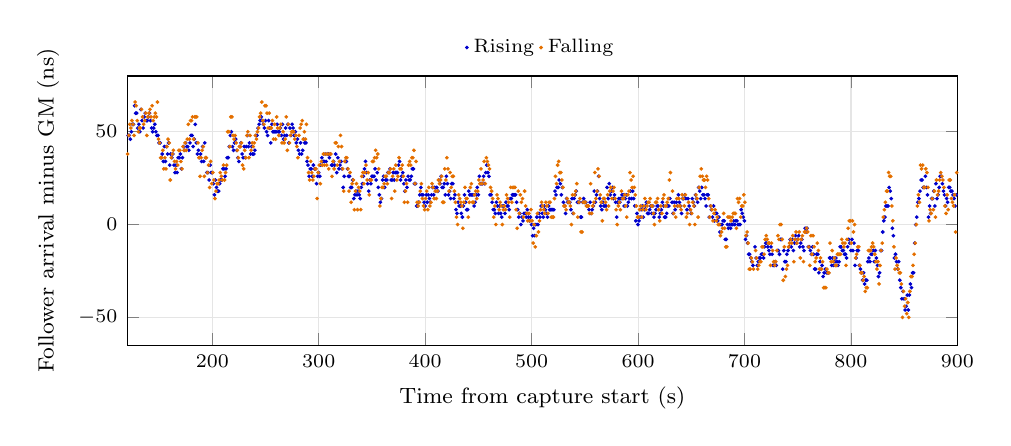
\begin{tikzpicture}
\begin{axis}[width=\columnwidth,height=5.0cm,tick label style={font=\scriptsize},label style={font=\footnotesize},grid=major,grid style={gray!20},xmin=120,xmax=900,ymin=-65,ymax=80,xlabel={Time from capture start (s)},ylabel={Follower arrival minus GM (ns)},legend style={font=\scriptsize,draw=none,at={(0.5,1.03)},anchor=south,legend columns=2}]
\addplot+[only marks,mark=*,mark size=.45pt,color=blue!80!black] coordinates {
(120.958408306,48.000000000)
(121.958281490,48.000000000)
(122.958154668,46.000000000)
(123.958027850,50.000000000)
(124.957901030,54.000000000)
(125.957774204,54.000000000)
(126.957647388,64.000000000)
(127.957520554,60.000000000)
(128.957393722,60.000000000)
(129.957266882,52.000000000)
(130.957140050,54.000000000)
(131.957013210,50.000000000)
(132.956886382,62.000000000)
(133.956759536,56.000000000)
(134.956632690,52.000000000)
(135.956505852,58.000000000)
(136.956379008,60.000000000)
(137.956252156,56.000000000)
(138.956125306,56.000000000)
(139.955998456,58.000000000)
(140.955871604,60.000000000)
(141.955744744,56.000000000)
(142.955617884,52.000000000)
(143.955491024,50.000000000)
(144.955364166,52.000000000)
(145.955237308,54.000000000)
(146.955110440,50.000000000)
(147.954983574,48.000000000)
(148.954856708,48.000000000)
(149.954729838,44.000000000)
(150.954602970,44.000000000)
(151.954476102,36.000000000)
(152.954349234,38.000000000)
(153.954222358,34.000000000)
(154.954095492,42.000000000)
(155.953968608,34.000000000)
(156.953841740,42.000000000)
(157.953714856,38.000000000)
(158.953587980,44.000000000)
(159.953461084,32.000000000)
(160.953334204,38.000000000)
(161.953207314,36.000000000)
(162.953080426,38.000000000)
(163.952953528,32.000000000)
(164.952826630,28.000000000)
(165.952699738,32.000000000)
(166.952572838,28.000000000)
(167.952445948,36.000000000)
(168.952319050,36.000000000)
(169.952192152,38.000000000)
(170.952065244,30.000000000)
(171.951938348,36.000000000)
(172.951811452,42.000000000)
(173.951684546,40.000000000)
(174.951557642,44.000000000)
(175.951430730,42.000000000)
(176.951303818,42.000000000)
(177.951176902,40.000000000)
(178.951049988,44.000000000)
(179.950923074,48.000000000)
(180.950796154,48.000000000)
(181.950669226,42.000000000)
(182.950542306,46.000000000)
(183.950415388,54.000000000)
(184.950288452,44.000000000)
(185.950161524,38.000000000)
(186.950034594,40.000000000)
(187.949907656,36.000000000)
(188.949780724,38.000000000)
(189.949653784,34.000000000)
(190.949526854,42.000000000)
(191.949399908,34.000000000)
(192.949272978,44.000000000)
(193.949146030,36.000000000)
(194.949019080,28.000000000)
(195.948892138,28.000000000)
(196.948765190,24.000000000)
(197.948638250,32.000000000)
(198.948511298,28.000000000)
(199.948384348,28.000000000)
(200.948257390,22.000000000)
(201.948130430,16.000000000)
(202.948003482,24.000000000)
(203.947876522,20.000000000)
(204.947749564,18.000000000)
(205.947622608,18.000000000)
(206.947495654,22.000000000)
(207.947368698,24.000000000)
(208.947241738,24.000000000)
(209.947114784,30.000000000)
(210.946987824,30.000000000)
(211.946860858,26.000000000)
(212.946733898,30.000000000)
(213.946606940,36.000000000)
(214.946479978,36.000000000)
(215.946353020,42.000000000)
(216.946226062,48.000000000)
(217.946099098,50.000000000)
(218.945972124,42.000000000)
(219.945845162,40.000000000)
(220.945718194,44.000000000)
(221.945591226,46.000000000)
(222.945464250,40.000000000)
(223.945337274,36.000000000)
(224.945210298,34.000000000)
(225.945083330,42.000000000)
(226.944956354,44.000000000)
(227.944829368,38.000000000)
(228.944702384,36.000000000)
(229.944575406,42.000000000)
(230.944448414,36.000000000)
(231.944321430,42.000000000)
(232.944194446,48.000000000)
(233.944067446,42.000000000)
(234.943940454,44.000000000)
(235.943813452,38.000000000)
(236.943686456,42.000000000)
(237.943559452,38.000000000)
(238.943432448,38.000000000)
(239.943305446,40.000000000)
(240.943178446,48.000000000)
(241.943051438,48.000000000)
(242.942924430,52.000000000)
(243.942797420,54.000000000)
(244.942670406,56.000000000)
(245.942543392,58.000000000)
(246.942416370,56.000000000)
(247.942289346,54.000000000)
(248.942162322,52.000000000)
(249.942035300,56.000000000)
(250.941908270,50.000000000)
(251.941781240,48.000000000)
(252.941654218,56.000000000)
(253.941527182,52.000000000)
(254.941400146,44.000000000)
(255.941273120,54.000000000)
(256.941146078,50.000000000)
(257.941019038,50.000000000)
(258.940891996,50.000000000)
(259.940764954,50.000000000)
(260.940637912,54.000000000)
(261.940510862,50.000000000)
(262.940383814,50.000000000)
(263.940256766,52.000000000)
(264.940129710,48.000000000)
(265.940002662,54.000000000)
(266.939875598,46.000000000)
(267.939748542,48.000000000)
(268.939621486,52.000000000)
(269.939494422,48.000000000)
(270.939367366,54.000000000)
(271.939240294,44.000000000)
(272.939113236,52.000000000)
(273.938986166,48.000000000)
(274.938859104,54.000000000)
(275.938732034,52.000000000)
(276.938604958,48.000000000)
(277.938477888,50.000000000)
(278.938350808,44.000000000)
(279.938223736,46.000000000)
(280.938096654,40.000000000)
(281.937969574,38.000000000)
(282.937842500,44.000000000)
(283.937715412,38.000000000)
(284.937588332,40.000000000)
(285.937461254,46.000000000)
(286.937334166,44.000000000)
(287.937207080,44.000000000)
(288.937079992,34.000000000)
(289.936952902,32.000000000)
(290.936825808,26.000000000)
(291.936698720,30.000000000)
(292.936571628,30.000000000)
(293.936444530,26.000000000)
(294.936317440,32.000000000)
(295.936190342,30.000000000)
(296.936063242,30.000000000)
(297.935936134,22.000000000)
(298.935809036,26.000000000)
(299.935681936,28.000000000)
(300.935554830,26.000000000)
(301.935427730,32.000000000)
(302.935300630,36.000000000)
(303.935173522,34.000000000)
(304.935046414,34.000000000)
(305.934919310,38.000000000)
(306.934792196,34.000000000)
(307.934665090,38.000000000)
(308.934537976,38.000000000)
(309.934410860,36.000000000)
(310.934283746,38.000000000)
(311.934156624,32.000000000)
(312.934029506,32.000000000)
(313.933902390,34.000000000)
(314.933775266,32.000000000)
(315.933648150,38.000000000)
(316.933521016,28.000000000)
(317.933393896,36.000000000)
(318.933266762,30.000000000)
(319.933139634,32.000000000)
(320.933012504,34.000000000)
(321.932885366,30.000000000)
(322.932758228,20.000000000)
(323.932631098,26.000000000)
(324.932503968,34.000000000)
(325.932376830,34.000000000)
(326.932249684,30.000000000)
(327.932122536,26.000000000)
(328.931995394,26.000000000)
(329.931868242,20.000000000)
(330.931741098,20.000000000)
(331.931613954,24.000000000)
(332.931486798,14.000000000)
(333.931359650,16.000000000)
(334.931232502,18.000000000)
(335.931105346,16.000000000)
(336.930978196,18.000000000)
(337.930851038,16.000000000)
(338.930723880,14.000000000)
(339.930596730,20.000000000)
(340.930469572,22.000000000)
(341.930342414,26.000000000)
(342.930215256,30.000000000)
(343.930088098,34.000000000)
(344.929960930,28.000000000)
(345.929833760,22.000000000)
(346.929706590,18.000000000)
(347.929579430,24.000000000)
(348.929452262,22.000000000)
(349.929325096,26.000000000)
(350.929197924,26.000000000)
(351.929070752,26.000000000)
(352.928943582,30.000000000)
(353.928816402,24.000000000)
(354.928689228,28.000000000)
(355.928562042,20.000000000)
(356.928434858,16.000000000)
(357.928307682,12.000000000)
(358.928180502,14.000000000)
(359.928053326,24.000000000)
(360.927926142,26.000000000)
(361.927798948,20.000000000)
(362.927671762,24.000000000)
(363.927544568,24.000000000)
(364.927417380,28.000000000)
(365.927290184,28.000000000)
(366.927162988,30.000000000)
(367.927035784,24.000000000)
(368.926908586,24.000000000)
(369.926781392,28.000000000)
(370.926654188,24.000000000)
(371.926526990,28.000000000)
(372.926399786,28.000000000)
(373.926272582,28.000000000)
(374.926145378,32.000000000)
(375.926018172,34.000000000)
(376.925890956,24.000000000)
(377.925763748,26.000000000)
(378.925636542,28.000000000)
(379.925509324,22.000000000)
(380.925382108,18.000000000)
(381.925254898,24.000000000)
(382.925127678,20.000000000)
(383.925000466,26.000000000)
(384.924873246,24.000000000)
(385.924746026,24.000000000)
(386.924618804,26.000000000)
(387.924491584,30.000000000)
(388.924364360,30.000000000)
(389.924237126,22.000000000)
(390.924109900,22.000000000)
(391.923982668,10.000000000)
(392.923855440,10.000000000)
(393.923728212,12.000000000)
(394.923600984,16.000000000)
(395.923473754,20.000000000)
(396.923346518,16.000000000)
(397.923219282,16.000000000)
(398.923092042,12.000000000)
(399.922964802,10.000000000)
(400.922837568,16.000000000)
(401.922710322,12.000000000)
(402.922583084,16.000000000)
(403.922455836,14.000000000)
(404.922328588,12.000000000)
(405.922201342,16.000000000)
(406.922074098,20.000000000)
(407.921946844,16.000000000)
(408.921819596,20.000000000)
(409.921692342,18.000000000)
(410.921565092,20.000000000)
(411.921437834,18.000000000)
(412.921310584,24.000000000)
(413.921183326,22.000000000)
(414.921056070,26.000000000)
(415.920928804,20.000000000)
(416.920801542,20.000000000)
(417.920674282,22.000000000)
(418.920547012,16.000000000)
(419.920419758,26.000000000)
(420.920292486,22.000000000)
(421.920165212,16.000000000)
(422.920037944,18.000000000)
(423.919910670,14.000000000)
(424.919783404,22.000000000)
(425.919656128,22.000000000)
(426.919528852,14.000000000)
(427.919401574,16.000000000)
(428.919274288,8.000000000)
(429.919147006,6.000000000)
(430.919019732,12.000000000)
(431.918892450,10.000000000)
(432.918765168,10.000000000)
(433.918637882,6.000000000)
(434.918510598,4.000000000)
(435.918383320,10.000000000)
(436.918256040,16.000000000)
(437.918128750,12.000000000)
(438.918001458,8.000000000)
(439.917874168,8.000000000)
(440.917746886,18.000000000)
(441.917619592,16.000000000)
(442.917492298,16.000000000)
(443.917365004,16.000000000)
(444.917237708,16.000000000)
(445.917110406,10.000000000)
(446.916983110,12.000000000)
(447.916855816,16.000000000)
(448.916728520,20.000000000)
(449.916601216,16.000000000)
(450.916473922,26.000000000)
(451.916346616,22.000000000)
(452.916219312,22.000000000)
(453.916092008,22.000000000)
(454.915964704,26.000000000)
(455.915837392,22.000000000)
(456.915710088,28.000000000)
(457.915582782,32.000000000)
(458.915455466,28.000000000)
(459.915328150,26.000000000)
(460.915200834,16.000000000)
(461.915073518,16.000000000)
(462.914946198,12.000000000)
(463.914818878,8.000000000)
(464.914691558,8.000000000)
(465.914564236,6.000000000)
(466.914436922,12.000000000)
(467.914309598,10.000000000)
(468.914182272,6.000000000)
(469.914054950,10.000000000)
(470.913927622,6.000000000)
(471.913800294,4.000000000)
(472.913672974,10.000000000)
(473.913545646,10.000000000)
(474.913418314,6.000000000)
(475.913290992,12.000000000)
(476.913163660,10.000000000)
(477.913036330,10.000000000)
(478.912908996,8.000000000)
(479.912781672,14.000000000)
(480.912654340,14.000000000)
(481.912527008,16.000000000)
(482.912399674,16.000000000)
(483.912272338,16.000000000)
(484.912145002,16.000000000)
(485.912017662,12.000000000)
(486.911890322,8.000000000)
(487.911762980,4.000000000)
(488.911635644,6.000000000)
(489.911508300,0E-9)
(490.911380964,4.000000000)
(491.911253622,2.000000000)
(492.911126286,6.000000000)
(493.910998944,6.000000000)
(494.910871608,4.000000000)
(495.910744268,8.000000000)
(496.910616918,4.000000000)
(497.910489568,2.000000000)
(498.910362224,4.000000000)
(499.910234872,0E-9)
(500.910107516,-6.000000000)
(501.909980170,-2.000000000)
(502.909852814,-6.000000000)
(503.909725468,0E-9)
(504.909598118,4.000000000)
(505.909470760,0E-9)
(506.909343410,6.000000000)
(507.909216050,4.000000000)
(508.909088698,10.000000000)
(509.908961336,6.000000000)
(510.908833974,4.000000000)
(511.908706618,10.000000000)
(512.908579256,8.000000000)
(513.908451892,6.000000000)
(514.908324528,4.000000000)
(515.908197170,10.000000000)
(516.908069804,8.000000000)
(517.907942436,8.000000000)
(518.907815068,8.000000000)
(519.907687700,8.000000000)
(520.907560330,8.000000000)
(521.907432968,18.000000000)
(522.907305592,16.000000000)
(523.907178220,20.000000000)
(524.907050846,20.000000000)
(525.906923472,24.000000000)
(526.906796092,22.000000000)
(527.906668708,16.000000000)
(528.906541332,20.000000000)
(529.906413950,12.000000000)
(530.906286566,10.000000000)
(531.906159178,6.000000000)
(532.906031800,14.000000000)
(533.905904412,12.000000000)
(534.905777024,12.000000000)
(535.905649636,12.000000000)
(536.905522244,8.000000000)
(537.905394860,14.000000000)
(538.905267460,6.000000000)
(539.905140076,14.000000000)
(540.905012684,16.000000000)
(541.904885292,18.000000000)
(542.904757890,12.000000000)
(543.904630492,12.000000000)
(544.904503094,12.000000000)
(545.904375686,4.000000000)
(546.904248286,4.000000000)
(547.904120894,12.000000000)
(548.903993494,14.000000000)
(549.903866092,12.000000000)
(550.903738690,12.000000000)
(551.903611284,10.000000000)
(552.903483882,10.000000000)
(553.903356474,8.000000000)
(554.903229072,12.000000000)
(555.903101658,6.000000000)
(556.902974250,8.000000000)
(557.902846842,10.000000000)
(558.902719438,18.000000000)
(559.902592018,12.000000000)
(560.902464606,16.000000000)
(561.902337194,18.000000000)
(562.902209784,26.000000000)
(563.902082364,14.000000000)
(564.901954942,10.000000000)
(565.901827520,8.000000000)
(566.901700104,12.000000000)
(567.901572682,10.000000000)
(568.901445260,10.000000000)
(569.901317838,10.000000000)
(570.901190424,20.000000000)
(571.901062994,14.000000000)
(572.900935576,22.000000000)
(573.900808144,16.000000000)
(574.900680718,18.000000000)
(575.900553292,20.000000000)
(576.900425856,14.000000000)
(577.900298428,16.000000000)
(578.900170992,12.000000000)
(579.900043552,4.000000000)
(580.899916128,12.000000000)
(581.899788696,14.000000000)
(582.899661258,12.000000000)
(583.899533824,14.000000000)
(584.899406390,16.000000000)
(585.899278954,16.000000000)
(586.899151510,10.000000000)
(587.899024074,14.000000000)
(588.898896636,16.000000000)
(589.898769190,10.000000000)
(590.898641750,12.000000000)
(591.898514310,14.000000000)
(592.898386870,18.000000000)
(593.898259420,14.000000000)
(594.898131980,18.000000000)
(595.898004528,14.000000000)
(596.897877076,10.000000000)
(597.897749630,2.000000000)
(598.897622186,6.000000000)
(599.897494730,0E-9)
(600.897367284,2.000000000)
(601.897239834,4.000000000)
(602.897112388,8.000000000)
(603.896984938,10.000000000)
(604.896857478,4.000000000)
(605.896730028,8.000000000)
(606.896602576,10.000000000)
(607.896475122,12.000000000)
(608.896347658,6.000000000)
(609.896220200,6.000000000)
(610.896092744,8.000000000)
(611.895965286,10.000000000)
(612.895837820,6.000000000)
(613.895710360,10.000000000)
(614.895582892,4.000000000)
(615.895455430,6.000000000)
(616.895327968,8.000000000)
(617.895200506,10.000000000)
(618.895073040,10.000000000)
(619.894945568,4.000000000)
(620.894818102,6.000000000)
(621.894690636,8.000000000)
(622.894563170,12.000000000)
(623.894435700,10.000000000)
(624.894308224,4.000000000)
(625.894180754,4.000000000)
(626.894053284,6.000000000)
(627.893925814,10.000000000)
(628.893798340,10.000000000)
(629.893670868,14.000000000)
(631.893415914,12.000000000)
(632.893288440,6.000000000)
(633.893160968,12.000000000)
(634.893033486,8.000000000)
(635.892906010,12.000000000)
(636.892778528,10.000000000)
(637.892651052,16.000000000)
(638.892523568,12.000000000)
(639.892396082,10.000000000)
(640.892268596,6.000000000)
(641.892141120,14.000000000)
(642.892013634,14.000000000)
(643.891886152,16.000000000)
(644.891758664,14.000000000)
(645.891631172,8.000000000)
(646.891503690,14.000000000)
(647.891376198,10.000000000)
(648.891248706,8.000000000)
(649.891121214,6.000000000)
(650.890993730,14.000000000)
(651.890866236,12.000000000)
(652.890738742,10.000000000)
(653.890611256,16.000000000)
(654.890483760,14.000000000)
(655.890356266,12.000000000)
(656.890228778,20.000000000)
(657.890101282,18.000000000)
(658.889973782,14.000000000)
(659.889846290,20.000000000)
(660.889718790,16.000000000)
(661.889591292,16.000000000)
(662.889463790,14.000000000)
(663.889336288,10.000000000)
(664.889208794,16.000000000)
(665.889081292,16.000000000)
(666.888953788,4.000000000)
(667.888826292,10.000000000)
(668.888698786,8.000000000)
(669.888571280,4.000000000)
(670.888443782,10.000000000)
(671.888316272,2.000000000)
(672.888188772,6.000000000)
(673.888061268,6.000000000)
(674.887933758,2.000000000)
(675.887806254,4.000000000)
(676.887678740,-4.000000000)
(677.887551236,0E-9)
(678.887423728,0E-9)
(679.887296222,2.000000000)
(680.887168712,2.000000000)
(681.887041192,-8.000000000)
(682.886913682,-8.000000000)
(683.886786178,0E-9)
(684.886658662,-2.000000000)
(685.886531150,0E-9)
(686.886403634,-2.000000000)
(687.886276120,0E-9)
(688.886148604,0E-9)
(689.886021088,2.000000000)
(690.885893568,0E-9)
(691.885766050,2.000000000)
(692.885638530,2.000000000)
(693.885511008,0E-9)
(694.885383486,0E-9)
(695.885255964,0E-9)
(696.885128450,8.000000000)
(697.885000924,6.000000000)
(698.884873400,4.000000000)
(699.884745874,2.000000000)
(700.884618348,-8.000000000)
(701.884490828,-6.000000000)
(702.884363300,-10.000000000)
(703.884235770,-16.000000000)
(704.884108248,-16.000000000)
(705.883980724,-18.000000000)
(706.883853198,-20.000000000)
(707.883725674,-22.000000000)
(709.883470636,-12.000000000)
(710.883343106,-18.000000000)
(711.883215576,-22.000000000)
(712.883088052,-20.000000000)
(713.882960526,-18.000000000)
(714.882833000,-18.000000000)
(715.882705474,-16.000000000)
(716.882577944,-16.000000000)
(717.882450412,-18.000000000)
(718.882322890,-12.000000000)
(719.882195360,-10.000000000)
(720.882067828,-10.000000000)
(721.881940294,-12.000000000)
(722.881812760,-14.000000000)
(723.881685224,-16.000000000)
(724.881557696,-12.000000000)
(725.881430158,-16.000000000)
(726.881302618,-22.000000000)
(727.881175084,-22.000000000)
(728.881047550,-20.000000000)
(729.880920014,-22.000000000)
(730.880792486,-14.000000000)
(731.880664950,-14.000000000)
(732.880537412,-16.000000000)
(733.880409882,-8.000000000)
(734.880282344,-8.000000000)
(735.880154798,-24.000000000)
(736.880027266,-14.000000000)
(737.879899718,-20.000000000)
(738.879772176,-20.000000000)
(739.879644634,-16.000000000)
(740.879517092,-14.000000000)
(741.879389548,-12.000000000)
(742.879262004,-8.000000000)
(743.879134452,-12.000000000)
(744.879006908,-8.000000000)
(745.878879354,-14.000000000)
(746.878751808,-10.000000000)
(747.878624260,-6.000000000)
(748.878496704,-10.000000000)
(749.878369154,-8.000000000)
(750.878241604,-6.000000000)
(751.878114046,-12.000000000)
(752.877986494,-10.000000000)
(753.877858942,-8.000000000)
(754.877731382,-12.000000000)
(755.877603826,-14.000000000)
(756.877476280,-2.000000000)
(757.877348722,-4.000000000)
(758.877221166,-2.000000000)
(759.877093600,-12.000000000)
(760.876966040,-12.000000000)
(761.876838480,-14.000000000)
(762.876710920,-16.000000000)
(763.876583364,-12.000000000)
(764.876455800,-16.000000000)
(765.876328234,-24.000000000)
(766.876200676,-24.000000000)
(767.876073126,-16.000000000)
(768.875945566,-16.000000000)
(769.875818004,-26.000000000)
(770.875690450,-20.000000000)
(771.875562886,-24.000000000)
(772.875435328,-22.000000000)
(773.875307760,-28.000000000)
(774.875180200,-26.000000000)
(775.875052640,-24.000000000)
(776.874925078,-26.000000000)
(777.874797516,-26.000000000)
(778.874669952,-26.000000000)
(779.874542396,-18.000000000)
(780.874414832,-18.000000000)
(781.874287264,-22.000000000)
(782.874159702,-18.000000000)
(783.874032132,-22.000000000)
(784.873904568,-20.000000000)
(785.873777004,-18.000000000)
(786.873649436,-20.000000000)
(787.873521868,-22.000000000)
(788.873394300,-20.000000000)
(789.873266740,-12.000000000)
(790.873139172,-12.000000000)
(791.873011600,-14.000000000)
(792.872884028,-14.000000000)
(793.872756454,-16.000000000)
(794.872628880,-16.000000000)
(795.872501304,-18.000000000)
(796.872373736,-12.000000000)
(797.872246164,-8.000000000)
(798.872118586,-10.000000000)
(799.871991006,-14.000000000)
(800.871863434,-8.000000000)
(801.871735850,-14.000000000)
(802.871608276,-10.000000000)
(803.871480694,-22.000000000)
(804.871353120,-18.000000000)
(805.871225544,-14.000000000)
(806.871097966,-14.000000000)
(807.870970378,-22.000000000)
(808.870842796,-24.000000000)
(809.870715212,-26.000000000)
(810.870587626,-30.000000000)
(811.870460048,-26.000000000)
(812.870332460,-32.000000000)
(813.870204878,-30.000000000)
(814.870077294,-30.000000000)
(815.869949720,-20.000000000)
(816.869822136,-18.000000000)
(817.869694548,-20.000000000)
(818.869566964,-16.000000000)
(819.869439378,-16.000000000)
(820.869311790,-14.000000000)
(821.869184196,-20.000000000)
(822.869056614,-14.000000000)
(823.868929020,-18.000000000)
(824.868801426,-22.000000000)
(825.868673830,-28.000000000)
(826.868546240,-26.000000000)
(827.868418660,-14.000000000)
(828.868291064,-14.000000000)
(829.868163478,-4.000000000)
(830.868035886,2.000000000)
(831.867908290,4.000000000)
(832.867780694,10.000000000)
(833.867653090,10.000000000)
(834.867525486,10.000000000)
(835.867397890,20.000000000)
(836.867270284,18.000000000)
(837.867142674,14.000000000)
(838.867015058,-2.000000000)
(839.866887448,-6.000000000)
(840.866759828,-18.000000000)
(841.866632220,-16.000000000)
(842.866504608,-20.000000000)
(843.866376992,-24.000000000)
(844.866249382,-20.000000000)
(845.866121760,-30.000000000)
(846.865994142,-34.000000000)
(847.865866522,-40.000000000)
(848.865738912,-36.000000000)
(849.865611294,-40.000000000)
(850.865483674,-46.000000000)
(851.865356062,-44.000000000)
(852.865228454,-38.000000000)
(853.865100832,-46.000000000)
(854.864973224,-38.000000000)
(855.864845614,-32.000000000)
(856.864717998,-34.000000000)
(857.864590390,-26.000000000)
(858.864462774,-26.000000000)
(859.864335172,-10.000000000)
(860.864207564,0E-9)
(861.864079950,4.000000000)
(862.863952340,12.000000000)
(863.863824720,14.000000000)
(864.863697102,18.000000000)
(865.863569486,24.000000000)
(866.863441862,24.000000000)
(867.863314236,20.000000000)
(868.863186610,20.000000000)
(869.863058990,26.000000000)
(870.862931358,20.000000000)
(871.862803728,16.000000000)
(872.862676096,4.000000000)
(873.862548474,10.000000000)
(874.862420842,6.000000000)
(875.862293220,14.000000000)
(876.862165590,14.000000000)
(877.862037962,18.000000000)
(878.861910324,10.000000000)
(879.861782704,22.000000000)
(880.861655064,14.000000000)
(881.861527432,16.000000000)
(882.861399804,20.000000000)
(883.861272176,26.000000000)
(884.861144542,26.000000000)
(885.861016906,22.000000000)
(886.860889268,18.000000000)
(887.860761630,16.000000000)
(888.860633990,10.000000000)
(889.860506358,14.000000000)
(890.860378720,12.000000000)
(891.860251090,20.000000000)
(892.860123452,20.000000000)
(893.859995812,18.000000000)
(894.859868172,18.000000000)
(895.859740530,16.000000000)
(896.859612888,14.000000000)
(897.859485244,10.000000000)
(898.859357608,16.000000000)
};
\addplot+[only marks,mark=*,mark size=.45pt,color=orange!90!black] coordinates {
(120.458471712,38.000000000)
(121.458344906,48.000000000)
(122.458218092,54.000000000)
(123.458091270,52.000000000)
(124.457964452,56.000000000)
(125.457837624,54.000000000)
(126.457710792,48.000000000)
(127.457583982,66.000000000)
(128.457457150,64.000000000)
(129.457330310,56.000000000)
(130.457203470,50.000000000)
(131.457076638,52.000000000)
(132.456949800,52.000000000)
(133.456822970,62.000000000)
(134.456696124,58.000000000)
(135.456569278,54.000000000)
(136.456442434,56.000000000)
(137.456315590,60.000000000)
(138.456188730,48.000000000)
(139.456061888,58.000000000)
(140.455935038,60.000000000)
(141.455808186,62.000000000)
(142.455681326,58.000000000)
(143.455554466,64.000000000)
(144.455427600,56.000000000)
(145.455300742,58.000000000)
(146.455173882,60.000000000)
(147.455047016,58.000000000)
(148.454920158,66.000000000)
(149.454793272,46.000000000)
(150.454666404,44.000000000)
(151.454539536,36.000000000)
(152.454412676,36.000000000)
(153.454285808,40.000000000)
(154.454158924,30.000000000)
(155.454032056,36.000000000)
(156.453905174,30.000000000)
(157.453778306,42.000000000)
(158.453651430,46.000000000)
(159.453524544,44.000000000)
(160.453397640,24.000000000)
(161.453270766,36.000000000)
(162.453143878,38.000000000)
(163.453016990,40.000000000)
(164.452890090,34.000000000)
(165.452763192,30.000000000)
(166.452636300,34.000000000)
(167.452509400,32.000000000)
(168.452382510,40.000000000)
(169.452255612,40.000000000)
(170.452128706,34.000000000)
(171.452001800,30.000000000)
(172.451874912,42.000000000)
(173.451748006,40.000000000)
(174.451621102,44.000000000)
(175.451494190,40.000000000)
(176.451367286,46.000000000)
(177.451240372,54.000000000)
(178.451113448,46.000000000)
(179.450986542,56.000000000)
(180.450859622,56.000000000)
(181.450732702,58.000000000)
(182.450605766,46.000000000)
(183.450478854,58.000000000)
(184.450351928,58.000000000)
(185.450225000,58.000000000)
(186.450098072,44.000000000)
(187.449971132,36.000000000)
(188.449844186,26.000000000)
(189.449717262,36.000000000)
(190.449590330,40.000000000)
(191.449463392,42.000000000)
(192.449336438,26.000000000)
(193.449209508,36.000000000)
(194.449082566,36.000000000)
(195.448955616,28.000000000)
(196.448828676,32.000000000)
(197.448701720,20.000000000)
(198.448574786,34.000000000)
(199.448447824,22.000000000)
(200.448320880,28.000000000)
(201.448193922,24.000000000)
(202.448066956,14.000000000)
(203.447940006,18.000000000)
(204.447813054,22.000000000)
(205.447686098,22.000000000)
(206.447559142,24.000000000)
(207.447432188,28.000000000)
(208.447305226,26.000000000)
(209.447178264,24.000000000)
(210.447051312,32.000000000)
(211.446924352,24.000000000)
(212.446797376,28.000000000)
(213.446670418,32.000000000)
(214.446543472,50.000000000)
(215.446416510,50.000000000)
(216.446289538,42.000000000)
(217.446162588,58.000000000)
(218.446035622,58.000000000)
(219.445908644,48.000000000)
(220.445781690,46.000000000)
(221.445654722,48.000000000)
(222.445527746,44.000000000)
(223.445400770,40.000000000)
(224.445273794,36.000000000)
(225.445146826,42.000000000)
(226.445019850,42.000000000)
(227.444892872,44.000000000)
(228.444765880,32.000000000)
(229.444638894,30.000000000)
(230.444511918,40.000000000)
(231.444384926,36.000000000)
(232.444257948,48.000000000)
(233.444130958,50.000000000)
(234.444003950,36.000000000)
(235.443876966,48.000000000)
(236.443749962,40.000000000)
(237.443622966,44.000000000)
(238.443495962,42.000000000)
(239.443368960,44.000000000)
(240.443241958,48.000000000)
(241.443114948,46.000000000)
(242.442987942,50.000000000)
(243.442860932,52.000000000)
(244.442733924,58.000000000)
(245.442606910,60.000000000)
(246.442479888,66.000000000)
(247.442352858,56.000000000)
(248.442225834,54.000000000)
(249.442098820,64.000000000)
(250.441971796,64.000000000)
(251.441844766,60.000000000)
(252.441717728,52.000000000)
(253.441590706,60.000000000)
(254.441463672,52.000000000)
(255.441336644,52.000000000)
(256.441209610,56.000000000)
(257.441082562,46.000000000)
(258.440955528,54.000000000)
(259.440828478,46.000000000)
(260.440701446,58.000000000)
(261.440574394,52.000000000)
(262.440447344,48.000000000)
(263.440320298,52.000000000)
(264.440193250,54.000000000)
(265.440066186,44.000000000)
(266.439939138,50.000000000)
(267.439812074,44.000000000)
(268.439685018,46.000000000)
(269.439557970,58.000000000)
(270.439430890,40.000000000)
(271.439303842,54.000000000)
(272.439176768,44.000000000)
(273.439049706,48.000000000)
(274.438922642,50.000000000)
(275.438795574,50.000000000)
(276.438668504,50.000000000)
(277.438541428,46.000000000)
(278.438414356,48.000000000)
(279.438287276,42.000000000)
(280.438160202,36.000000000)
(281.438033122,48.000000000)
(282.437906048,52.000000000)
(283.437778968,54.000000000)
(284.437651888,56.000000000)
(285.437524794,46.000000000)
(286.437397714,50.000000000)
(287.437270626,46.000000000)
(288.437143548,54.000000000)
(289.437016458,36.000000000)
(290.436889362,28.000000000)
(291.436762268,24.000000000)
(292.436635186,34.000000000)
(293.436508086,28.000000000)
(294.436380988,24.000000000)
(295.436253892,26.000000000)
(296.436126800,30.000000000)
(297.435999700,30.000000000)
(298.435872584,14.000000000)
(299.435745494,28.000000000)
(300.435618394,32.000000000)
(301.435491280,22.000000000)
(302.435364188,34.000000000)
(303.435237080,32.000000000)
(304.435109980,38.000000000)
(305.434982866,32.000000000)
(306.434855762,38.000000000)
(307.434728646,32.000000000)
(308.434601540,38.000000000)
(309.434474418,30.000000000)
(310.434347312,38.000000000)
(311.434220196,38.000000000)
(312.434093066,26.000000000)
(313.433965956,34.000000000)
(314.433838840,30.000000000)
(315.433711716,44.000000000)
(316.433584592,44.000000000)
(317.433457456,32.000000000)
(318.433330338,42.000000000)
(319.433203200,34.000000000)
(320.433076082,48.000000000)
(321.432948944,42.000000000)
(322.432821798,30.000000000)
(323.432694666,18.000000000)
(324.432567544,34.000000000)
(325.432440408,36.000000000)
(326.432313268,36.000000000)
(327.432186120,30.000000000)
(328.432058964,18.000000000)
(329.431931830,28.000000000)
(330.431804670,12.000000000)
(331.431677534,22.000000000)
(332.431550388,24.000000000)
(333.431423224,8.000000000)
(334.431296084,18.000000000)
(335.431168936,22.000000000)
(336.431041770,8.000000000)
(337.430914628,20.000000000)
(338.430787470,18.000000000)
(339.430660304,8.000000000)
(340.430533162,26.000000000)
(341.430406004,28.000000000)
(342.430278838,22.000000000)
(343.430151680,28.000000000)
(344.430024522,32.000000000)
(345.429897352,24.000000000)
(346.429770190,28.000000000)
(347.429643014,16.000000000)
(348.429515854,24.000000000)
(349.429388678,24.000000000)
(350.429261518,34.000000000)
(351.429134346,34.000000000)
(352.429007174,36.000000000)
(353.428880004,40.000000000)
(354.428752824,36.000000000)
(355.428625648,38.000000000)
(356.428498462,30.000000000)
(357.428371270,10.000000000)
(358.428244100,14.000000000)
(359.428116922,20.000000000)
(360.427989736,20.000000000)
(361.427862552,22.000000000)
(362.427735366,26.000000000)
(363.427608174,26.000000000)
(364.427480978,22.000000000)
(365.427353788,28.000000000)
(366.427226592,28.000000000)
(367.427099396,30.000000000)
(368.426972184,14.000000000)
(369.426844996,26.000000000)
(370.426717802,30.000000000)
(371.426590588,18.000000000)
(372.426463400,32.000000000)
(373.426336188,24.000000000)
(374.426208984,26.000000000)
(375.426081786,36.000000000)
(376.425954572,30.000000000)
(377.425827364,30.000000000)
(378.425700158,32.000000000)
(379.425572942,26.000000000)
(380.425445716,12.000000000)
(381.425318508,18.000000000)
(382.425191296,22.000000000)
(383.425064076,12.000000000)
(384.424936862,32.000000000)
(385.424809644,34.000000000)
(386.424682422,32.000000000)
(387.424555202,36.000000000)
(388.424427978,36.000000000)
(389.424300756,40.000000000)
(390.424173512,22.000000000)
(391.424046296,34.000000000)
(392.423919062,12.000000000)
(393.423791832,10.000000000)
(394.423664604,12.000000000)
(395.423537376,18.000000000)
(396.423410148,22.000000000)
(397.423282904,14.000000000)
(398.423155666,10.000000000)
(399.423028426,8.000000000)
(400.422901194,14.000000000)
(401.422773956,18.000000000)
(402.422646704,8.000000000)
(403.422519472,20.000000000)
(404.422392216,10.000000000)
(405.422264970,12.000000000)
(406.422137732,22.000000000)
(407.422010480,20.000000000)
(408.421883224,14.000000000)
(409.421755976,18.000000000)
(410.421628720,14.000000000)
(411.421501470,18.000000000)
(412.421374220,24.000000000)
(413.421246962,22.000000000)
(414.421119706,24.000000000)
(415.420992448,26.000000000)
(416.420865172,12.000000000)
(417.420737918,12.000000000)
(418.420610658,30.000000000)
(419.420483388,24.000000000)
(420.420356134,36.000000000)
(421.420228860,30.000000000)
(422.420101578,18.000000000)
(423.419974318,28.000000000)
(424.419847038,20.000000000)
(425.419719770,26.000000000)
(426.419592502,26.000000000)
(427.419465224,18.000000000)
(428.419337938,12.000000000)
(429.419210650,4.000000000)
(430.419083368,0E-9)
(431.418956104,16.000000000)
(432.418828820,14.000000000)
(433.418701536,12.000000000)
(434.418574252,10.000000000)
(435.418446958,-2.000000000)
(436.418319686,12.000000000)
(437.418192408,20.000000000)
(438.418065116,14.000000000)
(439.417937826,14.000000000)
(440.417810526,4.000000000)
(441.417683242,12.000000000)
(442.417555956,20.000000000)
(443.417428664,22.000000000)
(444.417301360,12.000000000)
(445.417174064,12.000000000)
(446.417046770,16.000000000)
(447.416919474,18.000000000)
(448.416792172,14.000000000)
(449.416664876,18.000000000)
(450.416537580,24.000000000)
(451.416410276,22.000000000)
(452.416282972,30.000000000)
(453.416155660,22.000000000)
(454.416028356,24.000000000)
(455.415901058,34.000000000)
(456.415773738,22.000000000)
(457.415646442,36.000000000)
(458.415519128,34.000000000)
(459.415391812,32.000000000)
(460.415264504,30.000000000)
(461.415137188,20.000000000)
(462.415009870,18.000000000)
(463.414882550,14.000000000)
(464.414755222,4.000000000)
(465.414627908,10.000000000)
(466.414500578,0E-9)
(467.414373272,16.000000000)
(468.414245948,14.000000000)
(469.414118618,8.000000000)
(470.413991298,12.000000000)
(471.413863970,10.000000000)
(472.413736634,0E-9)
(473.413609314,8.000000000)
(474.413481990,10.000000000)
(475.413354660,8.000000000)
(476.413227338,16.000000000)
(477.413100006,14.000000000)
(478.412972674,12.000000000)
(479.412845334,4.000000000)
(480.412718018,20.000000000)
(481.412590678,12.000000000)
(482.412463352,20.000000000)
(483.412336018,20.000000000)
(484.412208682,20.000000000)
(485.412081334,8.000000000)
(486.411953994,-2.000000000)
(487.411826662,18.000000000)
(488.411699312,6.000000000)
(489.411571984,16.000000000)
(490.411444640,12.000000000)
(491.411317304,14.000000000)
(492.411189954,4.000000000)
(493.411062626,18.000000000)
(494.410935276,10.000000000)
(495.410807944,6.000000000)
(496.410680596,2.000000000)
(497.410553254,6.000000000)
(498.410425902,2.000000000)
(499.410298560,8.000000000)
(500.410171206,2.000000000)
(501.410043844,-10.000000000)
(502.409916504,0E-9)
(503.409789140,-12.000000000)
(504.409661792,-6.000000000)
(505.409534450,6.000000000)
(506.409407084,-4.000000000)
(507.409279734,2.000000000)
(508.409152382,8.000000000)
(509.409025028,12.000000000)
(510.408897666,10.000000000)
(511.408770304,8.000000000)
(512.408642942,6.000000000)
(513.408515586,12.000000000)
(514.408388222,10.000000000)
(515.408260856,6.000000000)
(516.408133498,12.000000000)
(517.408006132,12.000000000)
(518.407878756,4.000000000)
(519.407751388,4.000000000)
(520.407624018,4.000000000)
(521.407496648,14.000000000)
(522.407369288,26.000000000)
(523.407241910,22.000000000)
(524.407114544,32.000000000)
(525.406987170,34.000000000)
(526.406859788,28.000000000)
(527.406732408,28.000000000)
(528.406605024,24.000000000)
(529.406477648,20.000000000)
(530.406350264,10.000000000)
(531.406222880,10.000000000)
(532.406095494,8.000000000)
(533.405968114,14.000000000)
(534.405840726,12.000000000)
(535.405713338,12.000000000)
(536.405585948,10.000000000)
(537.405458548,0E-9)
(538.405331172,16.000000000)
(539.405203772,6.000000000)
(540.405076388,16.000000000)
(541.404948996,18.000000000)
(542.404821604,22.000000000)
(543.404694190,4.000000000)
(544.404566800,12.000000000)
(545.404439402,14.000000000)
(546.404311986,-4.000000000)
(547.404184586,-4.000000000)
(548.404057200,12.000000000)
(549.403929800,12.000000000)
(550.403802398,12.000000000)
(551.403674994,10.000000000)
(552.403547590,10.000000000)
(553.403420186,10.000000000)
(554.403292776,6.000000000)
(555.403165376,22.000000000)
(556.403037952,6.000000000)
(557.402910546,10.000000000)
(558.402783136,12.000000000)
(559.402655740,28.000000000)
(560.402528312,14.000000000)
(561.402400900,18.000000000)
(562.402273496,30.000000000)
(563.402146084,26.000000000)
(564.402018664,16.000000000)
(565.401891242,12.000000000)
(566.401763812,2.000000000)
(567.401636404,14.000000000)
(568.401508982,14.000000000)
(569.401381560,12.000000000)
(570.401254132,8.000000000)
(571.401126716,16.000000000)
(572.400999284,10.000000000)
(573.400871868,18.000000000)
(574.400744442,20.000000000)
(575.400617008,14.000000000)
(576.400489582,18.000000000)
(577.400362154,20.000000000)
(578.400234718,14.000000000)
(579.400107280,8.000000000)
(580.399979840,0E-9)
(581.399852416,10.000000000)
(582.399724984,12.000000000)
(583.399597544,8.000000000)
(584.399470118,18.000000000)
(585.399342676,14.000000000)
(586.399215240,14.000000000)
(587.399087804,16.000000000)
(588.398960358,10.000000000)
(589.398832920,4.000000000)
(590.398705474,16.000000000)
(591.398578034,18.000000000)
(592.398450600,28.000000000)
(593.398323152,24.000000000)
(594.398195704,20.000000000)
(595.398068262,26.000000000)
(596.397940810,20.000000000)
(597.397813358,16.000000000)
(598.397685920,10.000000000)
(599.397558466,4.000000000)
(600.397431018,4.000000000)
(601.397303572,8.000000000)
(602.397176122,10.000000000)
(603.397048666,4.000000000)
(604.396921216,8.000000000)
(605.396793764,10.000000000)
(606.396666314,14.000000000)
(607.396538852,8.000000000)
(608.396411398,10.000000000)
(609.396283942,12.000000000)
(610.396156484,12.000000000)
(611.396029026,14.000000000)
(612.395901562,10.000000000)
(613.395774100,10.000000000)
(614.395646632,6.000000000)
(615.395519164,0E-9)
(616.395391712,12.000000000)
(617.395264248,12.000000000)
(618.395136784,14.000000000)
(619.395009312,8.000000000)
(620.394881840,2.000000000)
(621.394754380,10.000000000)
(622.394626906,6.000000000)
(623.394499446,14.000000000)
(624.394371970,16.000000000)
(625.394244494,10.000000000)
(626.394117022,10.000000000)
(627.393989552,12.000000000)
(628.393862080,14.000000000)
(629.393734616,24.000000000)
(630.393607144,28.000000000)
(632.393352190,18.000000000)
(633.393224708,6.000000000)
(634.393097234,10.000000000)
(635.392969750,4.000000000)
(636.392842278,14.000000000)
(637.392714794,10.000000000)
(638.392587318,14.000000000)
(639.392459832,10.000000000)
(640.392332346,8.000000000)
(641.392204870,16.000000000)
(642.392077384,14.000000000)
(643.391949896,10.000000000)
(644.391822416,16.000000000)
(645.391694918,4.000000000)
(646.391567434,6.000000000)
(647.391439952,12.000000000)
(648.391312452,0E-9)
(649.391184968,8.000000000)
(650.391057476,6.000000000)
(651.390929990,12.000000000)
(652.390802496,10.000000000)
(653.390674994,0E-9)
(654.390547516,16.000000000)
(655.390420022,14.000000000)
(656.390292518,4.000000000)
(657.390165038,20.000000000)
(658.390037540,26.000000000)
(659.389910048,30.000000000)
(660.389782548,26.000000000)
(661.389655048,24.000000000)
(662.389527550,24.000000000)
(663.389400046,20.000000000)
(664.389272552,26.000000000)
(665.389145050,24.000000000)
(666.389017540,14.000000000)
(667.388890044,4.000000000)
(668.388762546,10.000000000)
(669.388635042,8.000000000)
(670.388507534,2.000000000)
(671.388380034,6.000000000)
(672.388252534,8.000000000)
(673.388125024,2.000000000)
(674.387997522,4.000000000)
(675.387870010,0E-9)
(676.387742504,0E-9)
(677.387614992,-6.000000000)
(678.387487486,-4.000000000)
(679.387359978,-2.000000000)
(680.387232478,6.000000000)
(681.387104960,-2.000000000)
(682.386977440,-12.000000000)
(683.386849930,-12.000000000)
(684.386722432,4.000000000)
(685.386594918,4.000000000)
(686.386467404,4.000000000)
(687.386339888,2.000000000)
(688.386212374,4.000000000)
(689.386084858,6.000000000)
(690.385957340,6.000000000)
(691.385829822,6.000000000)
(692.385702302,-2.000000000)
(693.385574782,14.000000000)
(694.385447258,12.000000000)
(695.385319738,14.000000000)
(696.385192206,4.000000000)
(697.385064690,10.000000000)
(698.384937166,10.000000000)
(699.384809648,16.000000000)
(700.384682122,12.000000000)
(701.384554596,-6.000000000)
(702.384427076,-4.000000000)
(703.384299546,-10.000000000)
(704.384172008,-24.000000000)
(705.384044486,-24.000000000)
(706.383916970,-18.000000000)
(707.383789444,-20.000000000)
(708.383661918,-24.000000000)
(710.383406880,-14.000000000)
(711.383279350,-18.000000000)
(712.383151818,-24.000000000)
(713.383024294,-22.000000000)
(714.382896768,-20.000000000)
(715.382769240,-20.000000000)
(716.382641720,-12.000000000)
(717.382514190,-12.000000000)
(718.382386658,-16.000000000)
(719.382259136,-8.000000000)
(720.382131606,-6.000000000)
(721.382004072,-8.000000000)
(722.381876538,-10.000000000)
(723.381749004,-10.000000000)
(724.381621460,-22.000000000)
(725.381493938,-10.000000000)
(726.381366400,-14.000000000)
(727.381238852,-20.000000000)
(728.381111316,-22.000000000)
(729.380983782,-20.000000000)
(730.380856254,-14.000000000)
(731.380728726,-6.000000000)
(732.380601188,-8.000000000)
(733.380473658,0E-9)
(734.380346120,0E-9)
(735.380218582,-8.000000000)
(736.380091028,-30.000000000)
(737.379963504,-12.000000000)
(738.379835946,-28.000000000)
(739.379708406,-24.000000000)
(740.379580864,-22.000000000)
(741.379453328,-12.000000000)
(742.379325784,-10.000000000)
(743.379198238,-8.000000000)
(744.379070688,-10.000000000)
(745.378943142,-6.000000000)
(746.378815580,-20.000000000)
(747.378688042,-8.000000000)
(748.378560494,-4.000000000)
(749.378432936,-10.000000000)
(750.378305386,-8.000000000)
(751.378177836,-4.000000000)
(752.378050270,-18.000000000)
(753.377922726,-8.000000000)
(754.377795174,-6.000000000)
(755.377667604,-20.000000000)
(756.377540064,-4.000000000)
(757.377412508,-4.000000000)
(758.377284952,-2.000000000)
(759.377157394,-4.000000000)
(760.377029828,-12.000000000)
(761.376902268,-22.000000000)
(762.376774708,-6.000000000)
(763.376647138,-16.000000000)
(764.376519590,-6.000000000)
(765.376392024,-12.000000000)
(766.376264458,-20.000000000)
(767.376136902,-18.000000000)
(768.376009350,-10.000000000)
(769.375881788,-14.000000000)
(770.375754234,-24.000000000)
(771.375626680,-18.000000000)
(772.375499114,-24.000000000)
(773.375371556,-20.000000000)
(774.375243980,-34.000000000)
(775.375116420,-34.000000000)
(776.374988858,-34.000000000)
(777.374861306,-24.000000000)
(778.374733742,-26.000000000)
(779.374606178,-26.000000000)
(780.374478630,-10.000000000)
(781.374351056,-20.000000000)
(782.374223496,-14.000000000)
(783.374095924,-20.000000000)
(784.373968360,-18.000000000)
(785.373840790,-22.000000000)
(786.373713224,-22.000000000)
(787.373585664,-16.000000000)
(788.373458096,-16.000000000)
(789.373330528,-16.000000000)
(790.373202960,-16.000000000)
(791.373075398,-8.000000000)
(792.372947826,-10.000000000)
(793.372820252,-12.000000000)
(794.372692680,-10.000000000)
(795.372565104,-22.000000000)
(796.372437528,-8.000000000)
(797.372309958,-2.000000000)
(798.372182386,2.000000000)
(799.372054808,2.000000000)
(800.371927220,-10.000000000)
(801.371799654,2.000000000)
(802.371672070,-4.000000000)
(803.371544496,0E-9)
(804.371416916,-18.000000000)
(805.371289340,-16.000000000)
(806.371161764,-12.000000000)
(807.371034184,-12.000000000)
(808.370906594,-22.000000000)
(809.370779010,-26.000000000)
(810.370651428,-26.000000000)
(811.370523842,-30.000000000)
(812.370396262,-28.000000000)
(813.370268672,-36.000000000)
(814.370141090,-34.000000000)
(815.370013506,-34.000000000)
(816.369885940,-14.000000000)
(817.369758354,-14.000000000)
(818.369630768,-14.000000000)
(819.369503182,-12.000000000)
(820.369375596,-10.000000000)
(821.369248006,-12.000000000)
(822.369120414,-16.000000000)
(823.368992820,-20.000000000)
(824.368865226,-24.000000000)
(825.368737640,-20.000000000)
(826.368610036,-32.000000000)
(827.368482454,-22.000000000)
(828.368354870,-14.000000000)
(829.368227278,-10.000000000)
(830.368099686,4.000000000)
(831.367972092,8.000000000)
(832.367844496,12.000000000)
(833.367716900,18.000000000)
(834.367589296,18.000000000)
(835.367461700,28.000000000)
(836.367334094,26.000000000)
(837.367206488,26.000000000)
(838.367078874,10.000000000)
(839.366951266,2.000000000)
(840.366823646,-12.000000000)
(841.366696024,-24.000000000)
(842.366568422,-18.000000000)
(843.366440808,-22.000000000)
(844.366313192,-24.000000000)
(845.366185578,-26.000000000)
(846.366057964,-26.000000000)
(847.365930344,-32.000000000)
(848.365802712,-50.000000000)
(849.365675112,-36.000000000)
(850.365547492,-44.000000000)
(851.365419880,-40.000000000)
(852.365292258,-48.000000000)
(853.365164650,-42.000000000)
(854.365037028,-50.000000000)
(855.364909426,-36.000000000)
(856.364781818,-28.000000000)
(857.364654202,-28.000000000)
(858.364526592,-22.000000000)
(859.364398982,-16.000000000)
(860.364271372,-10.000000000)
(861.364143764,0E-9)
(862.364016154,10.000000000)
(863.363888540,16.000000000)
(864.363760922,12.000000000)
(865.363633304,32.000000000)
(866.363505680,30.000000000)
(867.363378058,32.000000000)
(868.363250422,20.000000000)
(869.363122796,20.000000000)
(870.362995182,30.000000000)
(871.362867552,28.000000000)
(872.362739918,20.000000000)
(873.362612288,2.000000000)
(874.362484666,8.000000000)
(875.362357034,6.000000000)
(876.362229412,14.000000000)
(877.362101776,8.000000000)
(878.361974154,18.000000000)
(879.361846510,4.000000000)
(880.361718896,24.000000000)
(881.361591256,16.000000000)
(882.361463626,18.000000000)
(883.361335998,24.000000000)
(884.361208370,28.000000000)
(885.361080734,26.000000000)
(886.360953098,24.000000000)
(887.360825460,20.000000000)
(888.360697814,10.000000000)
(889.360570174,6.000000000)
(890.360442550,16.000000000)
(891.360314904,8.000000000)
(892.360187282,24.000000000)
(893.360059644,24.000000000)
(894.359931996,14.000000000)
(895.359804354,12.000000000)
(896.359676712,10.000000000)
(897.359549078,16.000000000)
(898.359421424,-4.000000000)
(899.359293798,28.000000000)
};
\legend{Rising,Falling}
\end{axis}
\end{tikzpicture}
\caption{Independent digital PPS timing for fixed PI: all qualified post-cutoff edges, without phase filtering or skew correction. Two disturbed cycles and boundary partial pulses are excluded by the stated duration rule.}
\label{fig:pps}
\end{figure}
% END_PPS_FIGURE

The rising-edge range is -46 to +64 ns; the falling-edge range is -50 to +66 ns. The cutoff is applied to each edge time, explaining the one-pair count difference. No phase outlier rejection, smoothing, or detrending is used. The frequency command continues to change, so the cutoff does not establish stationary noise or thermal equilibrium. This physical observation complements the internal estimates for one PI run. It does not rank the other controllers, identify the origin of the mean bias, or establish calibrated accuracy.

Afterward, the operator moved only CH0 to share the grandmaster output feeding CH1, retaining the measurement leads and grounds. A 60.095-second same-source capture contains 61 rising-edge pairs with CH1-minus-CH0 mean +0.230 ns and range 0 to +2 ns; 60 falling pairs have mean +0.133 ns and range -2 to +2 ns. No extra transitions were detected in that short check. These empirical path differences are small compared with the PTP separation, but do not establish sub-nanosecond accuracy, explain the earlier disturbances, or calibrate the distinct TimeStick output paths. Shared-source loading differs from the baseline. No correction was applied. After restoring CH0 to the follower, a 30-second diagnostic still showed both PPS signals and uninterrupted locked serial exchanges, but revealed five short CH1 high segments followed by low notches near rising edges. Their cause remains undetermined. This diagnostic is archived separately. Investigation of the extra transitions and clean repeated captures remain necessary.

\subsection{Five-Controller PPS Campaign}
A later sequence on the same day repeated the five 300-second controller trials and the 900-second PI trial with simultaneous PPS and serial acquisition. All six firmware images matched the original R4 campaign hashes. The instrument, channel mapping, threshold preset, and sampling configuration were unchanged. The previously established pulse-duration rule was recorded in a campaign plan before outcome analysis; no phase-based selection or skew correction was added.

The sequence was PI, regression, adaptive PI, Kalman, PLL/FLL, and longer PI, with one observation per condition. Uploading each follower image restarted acquisition, and link loss caused grandmaster reinitialization between trials. Initial phases differed; this was not an experiment with identical imposed disturbances. For this campaign, the common 120-second cutoff starts at the Saleae capture origin for both PPS and approximately aligned serial observations. The original serial-only campaign instead measured that exclusion from its first accepted exchange.

The raw serial logs contain 2,334 accepted exchanges, with no sample-number gaps or reported exchange errors. All post-cutoff serial observations are in s3: 180 per short trial and 780 in the long trial. The longer PI record has 38.44 ns physical rising-edge RMS over 758 qualified pairs, alongside 38.16 ns internal RMS. These captures are retained separately from the earlier PI observation.

% BEGIN_PPS_SERVO_TABLE
\begin{table}[t]
\centering
\caption{Later simultaneous PPS and serial campaign. Values after 120 s from capture start; PPS uses qualified rising pairs. All timing values in ns.}
\label{tab:pps-servos}
\small
\setlength{\tabcolsep}{3pt}
\begin{tabular}{lrrrr}
\hline
Controller & Pairs & PPS mean & PPS RMS & Serial RMS \\
\hline
PI & 177 & -5.58 & 9.94 & 15.70 \\
Regression & 170 & +1.87 & 6.22 & 8.04 \\
Adaptive PI & 155 & +4.36 & 10.16 & 9.28 \\
Kalman & 159 & +4.96 & 11.55 & 9.80 \\
PLL/FLL & 176 & -7.98 & 17.77 & 23.81 \\
PI, 900 s & 758 & -8.31 & 38.44 & 38.16 \\
\hline
\end{tabular}
\end{table}
% END_PPS_SERVO_TABLE

Qualified PPS statistics in Table~\ref{tab:pps-servos} are conditional on the recorded pulse-duration exclusions. Brief extra transitions occurred in the grandmaster channel, and exclusion rates varied between trials. The archive includes raw transitions, every rejected segment, unmatched qualified edges, and separate physical and serial startup plots. A physical settling diagnostic requires a final in-band suffix of at least 30 seconds, with no gap greater than 1.5 seconds and observations reaching the capture end. Rejected pulses can prevent that criterion even while the serial controller remains locked; a missing settling result does not establish failure to converge. These single sequential observations extend the independent measurement to all five controllers, but do not establish a general ranking or identify the source of the extra transitions.

\section{Interpretation and Limitations}
The results support a limited but useful conclusion: both microcontroller architectures can host the compact protocol and servo implementations, and the R4 can sustain the tested direct-link campaign with inexpensive controller arithmetic. They do not show that a faster CPU improves physical synchronization. The peripheral clocks, link, controller settings, and environmental conditions determine the observed behavior alongside processing delay. Historical R3 runs and the R4 campaign used different conditions, so a causal processor comparison would require a new experiment.

In the original five-servo comparison, the same timestamp observations both drive and evaluate the servo. A small internal residual may coexist with physical PPS bias caused by directional delay, timestamp placement, peripheral output delay, or cable and instrument effects. Register readback establishes configuration, not time alignment. The PPS follow-ups provide an independent physical observable for all five controllers. Extra transitions, condition-dependent exclusions, residual fixture uncertainty, and lack of traceable calibration prevent an end-to-end accuracy claim. The lowest qualified RMS in the later short trials belongs to regression, whereas adaptive PI had the lowest internal RMS in the original campaign. This difference across sequential sessions reinforces the need for replicated comparisons under controlled conditions.

The control model also approximates the previous correction as applying over the full Sync interval. USB actuation latency is not estimated. The Kalman process and measurement covariances have not been identified from oscillator or link measurements, and the hybrid loop can lag changing frequency. None of the present results establishes holdover performance, resistance to packet-delay variation, or robustness against network load.

The platform remains a direct-link experimental subset. Broader use would require additional protocol functionality, conformance evaluation, recovery testing, and runtime-memory characterization. Initialization retries recovered the devices during bring-up, but that isolated observation is not proof of reliable recovery after arbitrary resets. No switch, competing traffic, cable-asymmetry sweep, or controlled thermal disturbance was included in the final campaign.

\section{Reproducibility and Next Measurements}
The experiment archive~\cite{artifact} associates raw serial logs with a capture manifest, firmware hashes, compile-size reports, extracted samples, and plotting tools. The firmware source is recorded at revision \texttt{530c8d12ea39}; the results were recorded at \texttt{ac6d0844de25}. The archive preserves interrupted attempts separately from the completed six-capture campaign. Eight native C++ suites, randomized protocol-input checks, and twenty-four Python analysis tests complement the hardware record. All seven examples compile for both architectures. These checks provide implementation evidence, not metrological calibration.

A stronger follow-up study should repeat the simultaneous PPS and serial measurement with a verified measurement path, documenting channel skew, cable delays, thresholds, instrument uncertainty, and warm-up. The present native recording, binary and CSV exports, raw serial logs, receipt timestamps, pulse exclusions, and SHA-256 hashes are retained in the October 16 archive. The first flat capture and subsequent startup capture are retained separately as bring-up evidence. Reversing channels and exchanging endpoint roles would help identify fixed biases. Repeated randomized servo trials should then use a common acquisition policy and comparable environmental conditions, with run-level uncertainty rather than treating correlated one-second samples as independent repeats.

Longer captures would support time-deviation and frequency-stability analysis over stated averaging intervals. Controlled phase steps, frequency disturbances, missed exchanges, background traffic, and disconnect/reconnect trials would separate acquisition, tracking, and recovery behavior. Stack high-water measurements and actuation-latency traces would address the remaining embedded-system limits. These measurements are proposed work, not results of the present campaign.

\section{Conclusion}
tinyPTP demonstrates a compact separation of software clock control from external Ethernet timestamping on Arduino UNO R3 and R4 Minima platforms. Five controllers fit the R3, while the R4 supports a larger receive buffer and microsecond-scale servo updates. The completed R4 campaign records 2,328 accepted exchanges; its longer PI record yields a 23.23 ns RMS internal offset after the common acquisition cutoff. The architecture and archived observations provide a basis for reproducible controller experiments. A separate 900-second physical capture gives 26.18 ns RMS rising-edge separation for 777 qualified post-cutoff pulse pairs, with two disturbed cycles explicitly excluded. A later simultaneous campaign measures all five controllers, yielding 6.22--17.77 ns qualified rising-edge RMS in its short trials. Measurement-path characterization, investigation of extra transitions, and controlled repeated trials are needed for an accuracy assessment or a general servo comparison.

\begin{thebibliography}{10}
\bibitem{ieee1588} IEEE, \emph{IEEE Standard for a Precision Clock Synchronization Protocol for Networked Measurement and Control Systems}, IEEE Std 1588-2019, 2020. \url{https://standards.ieee.org/ieee/1588/6825/}.
\bibitem{linuxptp} LinuxPTP Project, ``ptp4l(8),'' online documentation, accessed Oct. 15, 2026. \url{https://www.linuxptp.org/documentation/ptp4l/}.
\bibitem{giorgi} G. Giorgi and C. Narduzzi, ``Performance Analysis of Kalman-Filter-Based Clock Synchronization in IEEE 1588 Networks,'' \emph{IEEE Trans. Instrum. Meas.}, vol. 60, no. 8, pp. 2902--2909, 2011, doi: 10.1109/TIM.2011.2113120.
\bibitem{levine} J. Levine, ``Synchronizing Computer Clocks by the Use of Kalman Filters,'' NIST publication record, Nov. 14, 2011. \url{https://www.nist.gov/publications/synchronizing-computer-clocks-use-kalman-filters}.
\bibitem{timestick} Time Appliances Project, ``TimeStick,'' hardware and driver repository, revision \texttt{4c2935a1f723}, accessed Oct. 15, 2026. \url{https://github.com/Time-Appliances-Project/TimeStick}.
\bibitem{usbhost} USB Host Shield Library 2.0 contributors, ``USB Host Shield Library 2.0,'' version 1.7.0. \url{https://github.com/felis/USB_Host_Shield_2.0}.
\bibitem{max3421e} Analog Devices, ``MAX3421E: USB Peripheral/Host Controller with SPI Interface,'' product documentation, accessed Oct. 15, 2026. \url{https://www.analog.com/en/products/max3421e.html}.
\bibitem{r4} Arduino, ``UNO R4 Minima,'' hardware documentation, accessed Oct. 15, 2026. \url{https://docs.arduino.cc/hardware/uno-r4-minima/}.
\bibitem{saleae} Saleae, ``Logic Pro 8 Data Sheet,'' and ``Time Measurement Error,'' accessed Oct. 16, 2026. \url{https://downloads.saleae.com/specs/logic_pro_8_data_sheet.pdf}. \url{https://www.saleae.com/support/troubleshooting/capture-and-recording-issues/time-measurement-error}.
\bibitem{artifact} tinyPTP project, ``UNO R4 Minima port and hardware experiment,'' Oct. 2026, source and measurement archives, original servo results revision \texttt{ac6d0844de25}. Physical PPS follow-up dated Oct. 16, 2026. Repository access currently restricted. \url{https://github.com/ahmadexp/tinyPTP}.
\end{thebibliography}
\end{document}
